\documentclass{article}
\listfiles
\usepackage[
  a4paper,
  left=2cm, right=2cm,
  top=2cm, bottom=2cm
]{geometry}
\usepackage{graphicx} % Required for inserting images
\usepackage{amsmath}       % Équations avancées
\usepackage{amssymb}       % Symboles mathématiques
\usepackage{graphicx}      % Inclusion de figures
\usepackage{siunitx}       % Unités SI
\usepackage{setspace}
\singlespacing
\usepackage{multirow}
\usepackage{booktabs}      % Tableaux professionnels
\usepackage[table]{xcolor}
\usepackage{hyperref}      % Références cliquables
\usepackage[most]{tcolorbox}
\usepackage{bm}
\usepackage{float}

\usepackage[framemethod=TikZ]{mdframed}
\usepackage{pgfplots}  
\pgfplotsset{compat=1.17}
\usepackage{caption}   

\usepackage{enumitem}
\usepackage{titlesec}
\usepackage{wasysym}
\usepackage{tikz}
\usetikzlibrary{positioning,arrows.meta,shapes.geometric,decorations.pathreplacing,calc,3d,positioning,patterns} % pour "below=of ..." et "-Stealth"
\usepackage{tikz-3dplot}

\usepackage{algorithm}
\usepackage{algorithmic}

\usepackage{listings}
\usetikzlibrary{shapes,arrows,positioning,calc}

\usepackage{fancyvrb}
\usepackage{fvextra}
\usepackage{pifont}

\newcommand{\codeTight}{\fontsize{8pt}{9pt}\selectfont} 

\captionsetup{font=footnotesize,labelfont=bf,textfont=it,skip=0pt}

% Commandes personnalisées
\newcommand{\cmark}{\textcolor{successgreen}{\ding{51}}}
\newcommand{\xmark}{\textcolor{errorred}{\ding{55}}}
\newcommand{\wmark}{\textcolor{warningorange}{\ding{45}}}


% --- Espaces autour des flottants (tables, figures) ---
\setlength{\textfloatsep}{8pt plus 2pt minus 2pt}
\setlength{\floatsep}{8pt plus 2pt minus 2pt}
\setlength{\intextsep}{8pt plus 2pt minus 2pt}
\setlength{\abovecaptionskip}{4pt}
\setlength{\belowcaptionskip}{0pt}

% --- Listes pour tout le document ---
\setlist[itemize]{itemsep=0pt, topsep=2pt, parsep=0pt, partopsep=0pt}
\setlist[enumerate]{itemsep=0pt, topsep=2pt, parsep=0pt, partopsep=0pt}

% --- Espaces autour des titres ---
\titlespacing*{\section}
  {0pt}{2ex plus 1ex minus .2ex}{1ex plus .5ex minus .2ex}
\titlespacing*{\subsection}
  {0pt}{1.5ex plus .5ex minus .2ex}{0.7ex plus .3ex minus .1ex}

% --- Espaces autour des formules affichées ---
\setlength{\abovedisplayskip}{6pt}
\setlength{\belowdisplayskip}{6pt}
\setlength{\abovedisplayshortskip}{4pt}
\setlength{\belowdisplayshortskip}{4pt}

\definecolor{misty}{rgb}{1.0,0.89,0.88}
\definecolor{MyBlue}{rgb}{0.8,1.0,1.0}
\definecolor{Carnelian}{rgb}{0.7,0.11,0.11}
\definecolor{MyGreen}{rgb}{0.0,0.5,0.0}
\definecolor{MyGreen2}{rgb}{0.0,0.42,0.24}
\definecolor{corrigecolor}{RGB}{180,100,200}
\definecolor{methode1color}{RGB}{220,80,60}
\definecolor{methode2color}{RGB}{80,180,80}
\definecolor{lightblue}{RGB}{220,235,255}
\definecolor{successgreen}{RGB}{39,174,96}
\definecolor{warningorange}{RGB}{243,156,18}
\definecolor{errorred}{RGB}{231,76,60}
\definecolor{infoblue}{RGB}{52,152,219}
\definecolor{darkblue}{RGB}{44,62,80}
\definecolor{lightgray}{RGB}{245,245,245}
\definecolor{purple}{RGB}{142,68,173}
\definecolor{lightgray}{RGB}{245,245,245}
\definecolor{okgreen}{RGB}{39,174,96}
\definecolor{warnorange}{RGB}{230,126,34}

% Définition des couleurs
\definecolor{headercolor}{RGB}{70, 130, 180}
\definecolor{alphacolor}{RGB}{255, 100, 100}
\definecolor{gammacolor}{RGB}{100, 100, 255}
\definecolor{xraycolor}{RGB}{255, 200, 100}
\definecolor{electroncolor}{RGB}{100, 200, 100}
\definecolor{augercolor}{RGB}{200, 150, 255}
\definecolor{successcolor}{RGB}{34, 139, 34}



% Couleurs personnalisées
\definecolor{aircolor}{RGB}{200, 220, 255}
\definecolor{tungcolor}{RGB}{255, 220, 200}
\definecolor{ratiocolor}{RGB}{220, 255, 220}

% Couleurs personnalisées
\definecolor{aircolor}{RGB}{220, 220, 220}
\definecolor{tungcolor}{RGB}{255, 220, 200}
\definecolor{pmmacolor}{RGB}{200, 255, 200}
\definecolor{ratiocolor}{RGB}{200, 220, 255}


% Définition des couleurs
\definecolor{tungsten}{RGB}{100,100,120}
\definecolor{wpetg}{RGB}{80,80,100}
\definecolor{water}{RGB}{100,180,255}
\definecolor{waterlight}{RGB}{150,200,255}
\definecolor{source}{RGB}{255,200,0}
\definecolor{cone1}{RGB}{255,100,100}
\definecolor{cone2}{RGB}{100,100,255}

\definecolor{source}{RGB}{255,200,0}
\definecolor{cone20}{RGB}{100,150,255}
\definecolor{cone60}{RGB}{255,150,100}
\definecolor{water}{RGB}{100,180,255}


% Configuration des couleurs
\definecolor{typeA}{RGB}{231,76,60}
\definecolor{typeB}{RGB}{241,196,15}
\definecolor{typeC}{RGB}{230,126,34}
\definecolor{typeD0}{RGB}{155,89,182}
\definecolor{typeD1}{RGB}{52,152,219}
\definecolor{typeD2}{RGB}{26,188,156}
\definecolor{typeD3}{RGB}{46,204,113}
\definecolor{typeD4}{RGB}{149,165,166}

\definecolor{methode1}{RGB}{70,130,180}
\definecolor{methode1bis}{RGB}{60,179,113}
\definecolor{methode2}{RGB}{255,140,0}
\definecolor{theoriecolor}{RGB}{0,100,180}

% Couleurs
\definecolor{darkblue}{RGB}{0,51,102}
\definecolor{lightblue}{RGB}{230,240,250}
\definecolor{lightgreen}{RGB}{230,250,230}
\definecolor{lightorange}{RGB}{255,240,220}
\definecolor{lightred}{RGB}{255,230,230}
\definecolor{method1}{RGB}{70,130,180}
\definecolor{method1bis}{RGB}{60,179,113}
\definecolor{method2}{RGB}{255,140,0}

% Couleurs pour la figure
\definecolor{filtercolor}{RGB}{128,128,153}
\definecolor{containercolor}{RGB}{102,102,115}
\definecolor{watercolor}{RGB}{51,153,255}
\definecolor{prefiltercolor}{RGB}{0,255,0}
\definecolor{postfiltercolor}{RGB}{255,255,0}
\definecolor{precontainercolor}{RGB}{255,128,0}
\definecolor{postcontainercolor}{RGB}{128,0,128}
\definecolor{prewatercolor}{RGB}{0,255,255}
\definecolor{postwatercolor}{RGB}{255,0,255}


% Couleurs
\definecolor{sourcecolor}{RGB}{255, 50, 50}
\definecolor{conecolor}{RGB}{255, 150, 150}
\definecolor{pmmacolor}{RGB}{255, 180, 100}
\definecolor{watercolor}{RGB}{100, 150, 255}
\definecolor{usefulcolor}{RGB}{100, 200, 100}
\definecolor{lostcolor}{RGB}{200, 200, 200}
\definecolor{solidanglecolor}{RGB}{100, 200, 100}

% Couleurs personnalisées
\definecolor{sourcecolor}{RGB}{255,100,0}
\definecolor{matrixcolor}{RGB}{255,220,100}
\definecolor{upstreamcolor}{RGB}{100,100,255}
\definecolor{downstreamcolor}{RGB}{255,100,100}
\definecolor{watercolor}{RGB}{100,180,255}
\definecolor{conecolor}{RGB}{255,200,100}
\definecolor{aircolor}{RGB}{240,248,255}
\definecolor{warningcolor}{RGB}{255,150,0}
\definecolor{energie40}{RGB}{255,100,100}
\definecolor{energie122}{RGB}{255,150,50}
\definecolor{energie344}{RGB}{255,200,50}
\definecolor{energie779}{RGB}{150,200,50}
\definecolor{energie964}{RGB}{50,200,100}
\definecolor{energie1408}{RGB}{50,150,200}

% Couleurs personnalisées
\definecolor{airblue}{RGB}{135,206,250}
\definecolor{sourcemagenta}{RGB}{255,0,255}
\definecolor{conecolor}{RGB}{255,200,0}
\definecolor{kermacolor}{RGB}{0,255,255}
\definecolor{upstreamblue}{RGB}{0,0,255}
\definecolor{downstreamred}{RGB}{255,0,0}
\definecolor{slabcolor}{RGB}{255,255,0}
\definecolor{plaquecolor}{RGB}{100,200,100}
\definecolor{cone60color}{RGB}{100,200,100}
\definecolor{cone7color}{RGB}{255,150,150}

% Couleurs personnalisées
\definecolor{precontainer}{RGB}{255,165,0}
\definecolor{postcontainer}{RGB}{0,139,139}
\definecolor{backscatter}{RGB}{148,0,211}

% Définition des couleurs
\definecolor{pmma}{RGB}{255, 180, 120}
\definecolor{water}{RGB}{100, 180, 255}
\definecolor{tungsten}{RGB}{80, 80, 80}
\definecolor{container}{RGB}{180, 180, 180}
\definecolor{preplane}{RGB}{255, 150, 50}
\definecolor{postplane}{RGB}{160, 100, 220}
\definecolor{wpetg}{RGB}{140, 140, 160}

% Définition des couleurs
\definecolor{headercolor}{RGB}{70, 130, 180}
\definecolor{successcolor}{RGB}{34, 139, 34}
\definecolor{photocolor}{RGB}{255, 200, 200}
\definecolor{comptoncolor}{RGB}{200, 200, 255}
\definecolor{paircolor}{RGB}{200, 255, 200}

% Couleurs personnalisées
\definecolor{sourcecolor}{RGB}{255,100,100}
\definecolor{slabcolor}{RGB}{255,230,100}
\definecolor{upstreamcolor}{RGB}{100,150,255}
\definecolor{downstreamcolor}{RGB}{255,100,100}
\definecolor{kermacolor}{RGB}{100,255,255}
\definecolor{aircolor}{RGB}{220,240,255}
\definecolor{conecolor}{RGB}{255,200,150}
\definecolor{worldcolor}{RGB}{240,240,240}
\definecolor{envelopecolor}{RGB}{200,220,255}

\definecolor{transmitcolor}{RGB}{46,204,113}
\definecolor{absorbcolor}{RGB}{231,76,60}
\definecolor{scattercolor}{RGB}{241,196,15}
\definecolor{oldcolor}{RGB}{180,180,180}

% Couleurs personnalisées
\definecolor{aircolor}{RGB}{200,230,255}
\definecolor{watercolor}{RGB}{100,150,255}
\definecolor{sourcecolor}{RGB}{255,80,80}
\definecolor{detectorcolor}{RGB}{100,200,100}
\definecolor{conecolor}{RGB}{255,180,100}
\definecolor{cone7color}{RGB}{100,200,255}
\definecolor{envelopecolor}{RGB}{230,230,230}
\definecolor{upstreamcolor}{RGB}{80,80,255}
\definecolor{downstreamcolor}{RGB}{255,80,80}
\definecolor{gammacolor}{RGB}{255,200,0}

% Couleurs
\definecolor{spherecolor}{RGB}{100,150,255}
\definecolor{raycolor}{RGB}{255,100,100}
\definecolor{chordcolor}{RGB}{50,200,50}
\definecolor{centercolor}{RGB}{0,0,0}
\definecolor{pointcolor}{RGB}{200,50,50}

\definecolor{wpetg}{RGB}{34,139,34}      % Vert forêt pour W/PETG
\definecolor{inox}{RGB}{192,192,192}     % Gris argent pour Inox
\definecolor{water}{RGB}{100,149,237}    % Bleu pour eau
\definecolor{source}{RGB}{255,215,0}     % Or pour source
\definecolor{gamma}{RGB}{255,69,0}       % Orange-rouge pour gammas

% Couleurs
\definecolor{lightgreen}{RGB}{220,255,220}
\definecolor{lightyellow}{RGB}{255,255,220}
\definecolor{lightblue}{RGB}{220,235,255}
\definecolor{bismuth}{RGB}{180,140,200}
\definecolor{petg}{RGB}{200,200,220}
\definecolor{eau}{RGB}{150,200,255}
\definecolor{air}{RGB}{240,248,255}
\definecolor{cone60}{RGB}{255,200,150}

\definecolor{headerblue}{RGB}{41,128,185}
\definecolor{lightgray}{RGB}{245,245,245}

\definecolor{sourcecolor}{RGB}{255, 50, 50}
\definecolor{filtercolor}{RGB}{120, 120, 140}
\definecolor{containercolor}{RGB}{100, 100, 115}
\definecolor{pmmacolor}{RGB}{255, 180, 100}
\definecolor{watercolor}{RGB}{100, 150, 255}
\definecolor{tungstencolor}{RGB}{60, 60, 60}
\definecolor{precontainercolor}{RGB}{255, 140, 0}
\definecolor{postcontainercolor}{RGB}{150, 0, 150}
\definecolor{contactcolor}{RGB}{0, 200, 0}

% Boîtes colorées
\newtcolorbox{databox}[1]{
    colback=blue!5,
    colframe=blue!75!black,
    fonttitle=\bfseries,
    title=#1
}

\newtcolorbox{resultbox}[1]{
    colback=green!5,
    colframe=green!75!black,
    fonttitle=\bfseries,
    title=#1
}

\newtcolorbox{warningbox}[1]{
    colback=orange!5,
    colframe=orange!75!black,
    fonttitle=\bfseries,
    title=#1
}

% --- Espaces autour des flottants (tables, figures) ---
\setlength{\textfloatsep}{8pt plus 2pt minus 2pt}
\setlength{\floatsep}{8pt plus 2pt minus 2pt}
\setlength{\intextsep}{8pt plus 2pt minus 2pt}
\setlength{\abovecaptionskip}{4pt}
\setlength{\belowcaptionskip}{0pt}

% --- Listes pour tout le document ---
\setlist[itemize]{itemsep=0pt, topsep=2pt, parsep=0pt, partopsep=0pt}
\setlist[enumerate]{itemsep=0pt, topsep=2pt, parsep=0pt, partopsep=0pt}

% --- Espaces autour des titres ---
\titlespacing*{\section}
  {0pt}{2ex plus 1ex minus .2ex}{1ex plus .5ex minus .2ex}
\titlespacing*{\subsection}
  {0pt}{1.5ex plus .5ex minus .2ex}{0.7ex plus .3ex minus .1ex}

% --- Espaces autour des formules affichées ---
\setlength{\abovedisplayskip}{6pt}
\setlength{\belowdisplayskip}{6pt}
\setlength{\abovedisplayshortskip}{4pt}
\setlength{\belowdisplayshortskip}{4pt}

\title{
\vspace{-1cm}
{\color{blue}\rule{\linewidth}{2pt}}\\[0.5cm]
{\Huge\bfseries Simulation Monte Carlo Geant4}\\[0.3cm]
{\Large Effet d'une Plaque W/PETG sur le Débit de Dose}\\[0.3cm]
{\large Source Eur152 - Cône 60° -25 Millions d'Événements}\\[0.3cm]
{\color{Carnelian}\rule{\linewidth}{2pt}}
}
\title{\textbf{Calcul d'absorption de gamma dans de l'eau}\\[0.5cm]
\large Source Europium-152 -- Table de données NIST-- Code Python }
\author{Documentation technique}
\date{\today}

\begin{document}

\maketitle

\begin{abstract}
Ce document présente une série de calcul analytique d'absorption en utilisant les tables de données du NIST (coefficients d'absoption) et des codes simples python. Cela concerne les raies gamma et X de la source d'Europium d'une part, le spectre relatif d'emission du MiniX et finalement une approche pour la source d'Americium 241.
\end{abstract}

\newpage

\tableofcontents


%==============================================================================
\normalsize
\noindent \begin{mdframed}[backgroundcolor=orange!20]
\section{\Large \color{blue} \textbf{Signification des pourcentages d'absorption}\color{black}}
\end{mdframed}
\footnotesize
%==============================================================================

\begin{tcolorbox}[colback=blue!5,colframe=blue,title=\textbf{Définition}]
\noindent Le pourcentage d'absorption indiqué pour chaque raie représente la \color{blue}\textbf{fraction des photons de cette raie spécifique}\color{black} qui sont absorbés en traversant l'épaisseur d'eau indiquée.
\end{tcolorbox}

\begin{figure}[H]
\centering
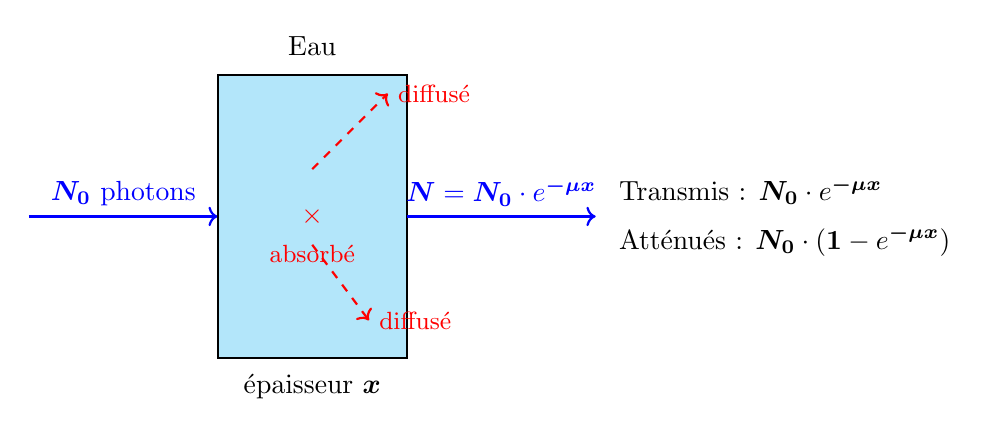
\begin{tikzpicture}[scale=1.2]
    % Faisceau incident
    \draw[->, thick, blue] (-3,0) -- (-1,0) node[midway, above] {$\bm{N_0}$ photons};
    
    % Bloc d'eau
    \fill[cyan!30] (-1,-1.5) rectangle (1,1.5);
    \draw[thick] (-1,-1.5) rectangle (1,1.5);
    \node at (0,1.8) {Eau};
    \node at (0,-1.8) {épaisseur $\bm{x}$};
    
    % Faisceau transmis
    \draw[->, thick, blue] (1,0) -- (3,0) node[midway, above] {$\bm{N} = \bm{N_0} \cdot e^{\bm{-\mu x}}$};
    
    % Photons absorbés/diffusés
    \draw[->, thick, red, dashed] (0,0.5) -- (0.8,1.3) node[right] {\small diffusé};
    \draw[->, thick, red, dashed] (0,-0.3) -- (0.6,-1.1) node[right] {\small diffusé};
    \node[red] at (0,0) {$\times$};
    \node[red, below] at (0,-0.2) {\small absorbé};
    
    % Légende
    \node[align=left] at (5,0) {
        Transmis : $\bm{N_0} \cdot e^{\bm{-\mu x}}$ \\[0.2cm]
        Atténués : $\bm{N_0} \cdot (\bm{1} - e^{\bm{-\mu x}})$
    };
\end{tikzpicture}
\captionsetup{labelformat=empty}
\caption{\footnotesize Atténuation d'un faisceau de photons dans l'eau}
\end{figure}

\begin{tcolorbox}[colback=blue!5,colframe=blue!75!black,title=\textbf{Attention}]

\noindent Le coefficient $\bm{\mu}$ (ou $\bm{\mu}/\bm{\rho}$) du NIST est le coefficient d'\color{blue}\textbf{atténuation totale}\color{black}, qui inclut plusieurs processus physiques :

\begin{enumerate}
    \item \color{blue}\textbf{Absorption photoélectrique}\color{black} : le photon disparaît complètement, son énergie est transférée à un électron
    \item \color{blue}\textbf{Diffusion Compton}\color{black} : le photon est dévié et perd une partie de son énergie
    \item \color{blue}\textbf{Diffusion cohérente (Rayleigh)}\color{black} : le photon est dévié sans perte d'énergie
    \item \color{blue}\textbf{Création de paires}\color{black} : (pour $\bm{E_\gamma }> 1.022$ MeV) le photon se convertit en paire $e^+/e^-$
\end{enumerate}

\vspace{0.3cm}

\noindent Donc \color{blue}\textbf{absorption}\color{black} \; dans ces tableaux signifie plus précisément \color{blue}\textbf{atténuation}\color{black} = photons retirés du faisceau direct, que ce soit par absorption vraie ou par diffusion.
\end{tcolorbox}

\begin{table}[H]
\centering
\begin{tabular}{@{}l l@{}}
\toprule
\footnotesize \textbf{Grandeur} &\footnotesize  \textbf{Formule} \\
\midrule
\footnotesize Photons transmis &\footnotesize  $\bm{N} = \bm{N_0} \cdot e^{\bm{-\mu x}}$ \\[0.3cm]
\footnotesize Photons atténués &\footnotesize  $\bm{N}_{\text{att}} = \bm{N_0} \cdot (\bm{1} - e^{\bm{-\mu x}})$ \\[0.3cm]
\footnotesize Fraction transmise &\footnotesize  $\bm{T} = e^{-\bm{\mu x}}$ \\[0.3cm]
\footnotesize Fraction atténuée (absorption) &\footnotesize  $\bm{A} = \bm{1} - e^{-\bm{\mu x}}$ \\[0.3cm]
\footnotesize Épaisseur de demi-atténuation &\footnotesize  $\bm{x_{1/2}} = \dfrac{\ln 2}{\bm{\mu}}$ \\[0.4cm]
\footnotesize Épaisseur pour 90\% d'atténuation &\footnotesize  $\bm{x_{90}} = \dfrac{\ln \bm{10}}{\bm{\mu}}$ \\
\bottomrule
\end{tabular}
\captionsetup{labelformat=empty}
\caption{Formules d'atténuation des photons}
\end{table}

\noindent L'absorption est calculée par la \color{blue}\textbf{loi de Beer-Lambert}\color{black} :

\begin{equation*}
\bm{\text{Absorption (\%)}} = \left[\bm{1} - e^{-\bm{\mu} \cdot \bm{x}}\right] \times \bm{100}
\end{equation*}

\noindent où :

\begin{itemize}
    \item $\bm{\mu}$ = coefficient d'atténuation linéaire (cm$^{-1}$)
    \item $\bm{x}$ = épaisseur d'eau (cm)
\end{itemize}

\noindent  Le coefficient d'atténuation linéaire est obtenu à partir du coefficient massique :

\begin{equation*}
\bm{\mu} = \frac{\bm{\mu}}{\bm{\rho}} \times \bm{\rho}
\end{equation*}

\noindent Pour l'eau, $\bm{\rho} = \bm{1}$ g/cm$^3$, donc numériquement $\bm{\mu} = \bm{\mu}/\bm{\rho}$.

\noindent Pour la raie 59.54 keV, épaisseur 5 mm :
\medskip

\begin{itemize}
    \item \textbf{Absorption = 9.8\%} signifie :
    \begin{itemize}
        \item Sur 100 photons de 59.54 keV émis par la source
        \item \textbf{9.8 photons} sont absorbés dans les 5 mm d'eau
        \item \textbf{90.2 photons} traversent sans être absorbés
    \end{itemize}
\end{itemize}
\medskip
\noindent La moyenne pondérée tient compte de l'intensité relative $\bm{I_i}$ de chaque raie :

\begin{equation*}
\bm{\text{Absorption moyenne}} = \frac{\displaystyle\bm{\sum_i} \left(\bm{\text{Abs}_i} \times \bm{I_i}\right)}{\displaystyle\bm{\sum_i} \bm{I_i}}
\end{equation*}

\noindent C'est donc l'absorption globale qu'on observerait si on considérait tous les photons émis par la source, en tenant compte du fait que certaines raies sont plus intenses que d'autres.


\clearpage

%==============================================================================
\normalsize
\noindent \begin{mdframed}[backgroundcolor=orange!20]
\section{\Large \color{blue} \textbf{Tableau des épaisseurs d'eau pour 90$\%$ d'absorption - Raies Eu-152}\color{black}}
\end{mdframed}
\footnotesize
%==============================================================================


\begin{table}[H]
\centering
\captionsetup{labelformat=empty}
\caption{\footnotesize Épaisseur d'eau nécessaire pour absorber 90\% des photons $\gamma$ de l'Eu-152}
\begin{tabular}{@{}c c c c c c@{}}
\toprule
\footnotesize\textbf{Raie} &\footnotesize \textbf{Énergie} &\footnotesize \textbf{Intensité} &\footnotesize $\bm{\mu/\rho}$ &\footnotesize $\bm{\mu}$ &\footnotesize $\bm{x_{90}}$ \\
 &\footnotesize (keV) &\footnotesize (\%) &\footnotesize (cm$^2$/g) &\footnotesize (cm$^{-1}$) & (mm) \\
\midrule
\footnotesize40 keV (X) &\footnotesize 39.52 &\footnotesize 20.78 &\footnotesize 0.2721 &\footnotesize 0.2721 &\footnotesize 84.6 \\
\footnotesize40 keV (X) &\footnotesize 40.12 &\footnotesize 37.72 &\footnotesize 0.2677 &\footnotesize 0.2677 &\footnotesize 86.0 \\
\rowcolor{yellow!20}
\footnotesize122 keV &\footnotesize 121.78 &\footnotesize 28.41 &\footnotesize 0.1606 &\footnotesize 0.1606 &\footnotesize 143.4 \\
\footnotesize245 keV &\footnotesize 244.70 &\footnotesize 7.53 &\footnotesize 0.1275 &\footnotesize 0.1275 &\footnotesize 180.6 \\
\rowcolor{yellow!20}
\footnotesize344 keV &\footnotesize 344.28 &\footnotesize 26.59 &\footnotesize 0.1124 &\footnotesize 0.1124 &\footnotesize 204.8 \\
\footnotesize411 keV &\footnotesize 411.12 &\footnotesize 2.23 &\footnotesize 0.1049 &\footnotesize 0.1049 &\footnotesize 219.5 \\
\footnotesize444 keV &\footnotesize 443.96 &\footnotesize 2.83 &\footnotesize 0.1017 &\footnotesize 0.1017 &\footnotesize 226.4 \\
\footnotesize779 keV &\footnotesize 778.90 &\footnotesize 12.97 &\footnotesize 0.0796 &\footnotesize 0.0796 &\footnotesize 289.3 \\
\footnotesize867 keV &\footnotesize 867.38 &\footnotesize 4.24 &\footnotesize 0.0757 &\footnotesize 0.0757 &\footnotesize 304.3 \\
\rowcolor{yellow!20}
\footnotesize964 keV &\footnotesize 964.08 &\footnotesize 14.63 &\footnotesize 0.0720 &\footnotesize 0.0720 &\footnotesize 320.0 \\
\footnotesize1086 keV &\footnotesize 1085.84 &\footnotesize 10.21 &\footnotesize 0.0679 &\footnotesize 0.0679 &\footnotesize 339.3 \\
\rowcolor{yellow!20}
\footnotesize1112 keV &\footnotesize 1112.07 &\footnotesize 13.64 &\footnotesize 0.0670 &\footnotesize 0.0670 &\footnotesize 343.4 \\
\rowcolor{yellow!20}
\footnotesize1408 keV &\footnotesize 1408.01 &\footnotesize 20.87 &\footnotesize 0.0595 &\footnotesize 0.0595 &\footnotesize 387.3 \\
\bottomrule
\end{tabular}

\vspace{0.1cm}
\footnotesize
\textbf{Notes :} Formule : $x_{90} = \ln(10) / \mu = 2.303 / \mu$, $\mu = (\mu/\rho) \times \rho$ avec $\rho_{\text{eau}} = 1$ g/cm$^3$, Coefficients $\mu/\rho$ interpolés des données NIST XCOM, Lignes surlignées : raies principales ($I > 10\%$)
\end{table}

%===============================================================================
\normalsize
\noindent \begin{mdframed}[backgroundcolor=orange!20]
\subsection{\color{blue}\textbf{Tableau comparatif avec différents taux d'absorption}\color{black}}
\end{mdframed}
\footnotesize
%===============================================================================
\medskip

\begin{table}[H]
\centering
\captionsetup{labelformat=empty}
\caption{\footnotesize Épaisseur d'eau pour différents taux d'absorption}
\begin{tabular}{@{}c c c c c@{}}
\toprule
\footnotesize \textbf{Raie} &\footnotesize $\bm{x_{50}}$ &\footnotesize $\bm{x_{90}}$ &\footnotesize $\bm{x_{99}}$ &\footnotesize $\bm{x_{99.9}}$ \\
\footnotesize (keV) &\footnotesize (mm) &\footnotesize (mm) &\footnotesize (mm) &\footnotesize (mm) \\
\midrule
\footnotesize 40 (X) &\footnotesize 25.5 &\footnotesize 84.6 & 169.2 & 253.9 \\
\footnotesize 40 (X) &\footnotesize 25.9 &\footnotesize 86.0 &\footnotesize 172.0 &\footnotesize 258.0 \\
\footnotesize 122 &\footnotesize 43.2 &\footnotesize 143.4 &\footnotesize 286.8 &\footnotesize 430.2 \\
\footnotesize 245 &\footnotesize 54.4 &\footnotesize 180.6 &\footnotesize 361.1 &\footnotesize 541.7 \\
\footnotesize 344 &\footnotesize 61.6 &\footnotesize 204.8 &\footnotesize 409.6 &\footnotesize 614.3 \\
\footnotesize 411 &\footnotesize 66.1 &\footnotesize 219.5 &\footnotesize 438.9 &\footnotesize 658.4 \\
\footnotesize 444 &\footnotesize 68.2 &\footnotesize 226.4 &\footnotesize 452.9 &\footnotesize 679.3 \\
\footnotesize 779 &\footnotesize 87.1 &\footnotesize 289.3 &\footnotesize 578.5 &\footnotesize 867.8 \\
\footnotesize 867 &\footnotesize 91.6 &\footnotesize 304.3 &\footnotesize 608.5 &\footnotesize 912.8 \\
\footnotesize 964 &\footnotesize 96.3 &\footnotesize 320.0 &\footnotesize 639.9 &\footnotesize 959.9 \\
\footnotesize 1086 &\footnotesize 102.1 &\footnotesize 339.3 &\footnotesize 678.7 &\footnotesize 1018.0 \\
\footnotesize 1112 &\footnotesize 103.4 &\footnotesize 343.4 &\footnotesize 686.8 &\footnotesize 1030.2 \\
\footnotesize 1408 &\footnotesize 116.6 &\footnotesize 387.3 &\footnotesize 774.6 &\footnotesize 1161.9 \\
\bottomrule
\end{tabular}
\medskip
\end{table}
\footnotesize
\noindent \textbf{Formules :} $x_{50} = \ln(2) / \mu$ \quad (demi-atténuation), $x_{90} = \ln(10) / \mu$, $x_{99} = \ln(100) / \mu$, $x_{99.9} = \ln(1000) / \mu$

\clearpage

%===============================================================================
\normalsize
\noindent \begin{mdframed}[backgroundcolor=orange!20]
\subsection{\color{blue}\textbf{Comparaison avec la simulation (5 mm d'eau)}\color{black}}
\end{mdframed}
 %===============================================================================
\medskip

\begin{table}[H]
\centering
\captionsetup{labelformat=empty}
\caption{\footnotesize Comparaison avec la simulation (épaisseur d'eau = 5 mm)}
\begin{tabular}{@{}c c c c c@{}}
\toprule
\footnotesize \textbf{Raie} &\footnotesize $\bm{\mu}$ &\footnotesize \textbf{Absorption} &\footnotesize $\bm{x_{90}}$ &\footnotesize \textbf{Facteur} \\
\footnotesize (keV) &\footnotesize (cm$^{-1}$) &\footnotesize \textbf{dans 5 mm (\%)} &\footnotesize (mm) &\footnotesize $\bm{x_{90}/5}$ \\
\midrule
\footnotesize 40 (X) &\footnotesize 0.2721 &\footnotesize12.72 &\footnotesize 84.6 &\footnotesize 16.9× \\
\footnotesize 40 (X) &\footnotesize 0.2677 &\footnotesize 12.53 &\footnotesize 86.0 &\footnotesize 17.2× \\
\footnotesize 122 &\footnotesize 0.1606 &\footnotesize 7.71 &\footnotesize 143.4 &\footnotesize 28.7× \\
\footnotesize 245 &\footnotesize 0.1275 &\footnotesize 6.18 &\footnotesize 180.6 &\footnotesize 36.1× \\
\footnotesize 344 &\footnotesize 0.1124 &\footnotesize 5.47 &\footnotesize 204.8 &\footnotesize 41.0× \\
\footnotesize 411 &\footnotesize 0.1049 &\footnotesize 5.11 &\footnotesize 219.5 &\footnotesize 43.9× \\
\footnotesize 444 &\footnotesize 0.1017 &\footnotesize 4.96 &\footnotesize 226.4 &\footnotesize 45.3× \\
\footnotesize 779 &\footnotesize 0.0796 &\footnotesize 3.90 &\footnotesize 289.3 &\footnotesize 57.9× \\
\footnotesize 867 &\footnotesize 0.0757 &\footnotesize 3.71 &\footnotesize 304.3 &\footnotesize 60.9× \\
\footnotesize 964 &\footnotesize 0.0720 &\footnotesize 3.53 &\footnotesize 320.0 &\footnotesize 64.0× \\
\footnotesize 1086 &\footnotesize 0.0679 & \footnotesize3.34 &\footnotesize 339.3 &\footnotesize 67.9× \\
\footnotesize 1112 &\footnotesize 0.0670 &\footnotesize 3.30 &\footnotesize 343.4 &\footnotesize 68.7× \\
\footnotesize 1408 &\footnotesize 0.0595 &\footnotesize 2.93 &\footnotesize 387.3 &\footnotesize 77.5× \\
\bottomrule
\end{tabular}

\vspace{0.1cm}
\footnotesize
\textbf{Absorption dans 5 mm :} $1 - \exp(-\mu \times 0.5)$
\end{table}

%===============================================================================
% Encadré de synthèse
%===============================================================================

\begin{tcolorbox}[colback=blue!5,colframe=blue,title=\textbf{Synthèse}]
\footnotesize
\noindent \textbf{Pour absorber 90\% des photons de l'Eu-152 :}
\begin{itemize}
    \item Rayons X (40 keV) : $x_{90} \approx$ \textbf{8.5 cm} d'eau
    \item Raie 122 keV : $x_{90} \approx$ \textbf{14.3 cm} d'eau
    \item Raie 344 keV : $x_{90} \approx$ \textbf{20.5 cm} d'eau
    \item Raie 1408 keV : $x_{90} \approx$ \textbf{38.7 cm} d'eau
\end{itemize}

\noindent \textbf{Avec 5 mm d'eau (simulation actuelle) :}
\begin{itemize}
    \item Absorption globale : $\sim$0.7\% (cohérent avec simulation : 0.73\%)
    \item Il faudrait \textbf{17× à 78× plus d'eau} selon la raie pour atteindre 90\%
\end{itemize}
\end{tcolorbox}

\clearpage

%==============================================================================
\normalsize
\noindent \begin{mdframed}[backgroundcolor=orange!20]
\section{\Large \color{blue} \textbf{Tableau du pourcentage d'absorption des raies Eu-152 dans l'eau 
Épaisseurs : 3 mm, 5 mm, 10 mm}\color{black}}
\end{mdframed}
\footnotesize
%==============================================================================


\begin{table}[H]
\centering
\captionsetup{labelformat=empty}
\caption{\footnotesize Pourcentage d'absorption des raies $\gamma$ de l'Eu-152 dans l'eau}
\begin{tabular}{@{}l c c c c c c@{}}
\toprule
\footnotesize \textbf{Raie} &\footnotesize \textbf{Énergie} &\footnotesize \textbf{Intensité} &\footnotesize $\bm{\mu/\rho}$ &\footnotesize \textbf{Abs. 3mm} &\footnotesize \textbf{Abs. 5mm} &\footnotesize \textbf{Abs. 10mm} \\
 &\footnotesize (keV) \footnotesize (\%) &\footnotesize (cm$^2$/g) &\footnotesize (\%) &\footnotesize (\%) &\footnotesize (\%) \\
\midrule
\rowcolor{yellow!20} \footnotesize 40 keV (X) &\footnotesize 39.52 &\footnotesize 20.78 &\footnotesize 0.2721 &\footnotesize 7.84 &\footnotesize 12.72 &\footnotesize 23.82 \\
\rowcolor{yellow!20} \footnotesize 40 keV (X) &\footnotesize 40.12 &\footnotesize 37.72 &\footnotesize 0.2677 &\footnotesize 7.72 &\footnotesize 12.53 &\footnotesize 23.49 \\
\rowcolor{yellow!20} \footnotesize 122 keV &\footnotesize 121.78 &\footnotesize 28.41 &\footnotesize 0.1606 &\footnotesize 4.70 &\footnotesize 7.71 &\footnotesize 14.83 \\
\footnotesize 245 keV &\footnotesize 244.70 &\footnotesize 7.53 &\footnotesize 0.1275 &\footnotesize 3.75 &\footnotesize 6.18 &\footnotesize 11.97 \\
\rowcolor{yellow!20} \footnotesize344 keV &\footnotesize 344.28 &\footnotesize 26.59 &\footnotesize 0.1124 &\footnotesize 3.32 &\footnotesize 5.47 &\footnotesize 10.64 \\
\footnotesize 411 keV &\footnotesize 411.12 &\footnotesize 2.23 &\footnotesize 0.1049 &\footnotesize 3.10 &\footnotesize 5.11 &\footnotesize 9.96 \\
\footnotesize 444 keV &\footnotesize 443.96 &\footnotesize 2.83 &\footnotesize 0.1017 &\footnotesize 3.00 &\footnotesize 4.96 &\footnotesize 9.67 \\
\footnotesize 779 keV &\footnotesize 778.90 &\footnotesize 12.97 &\footnotesize 0.0796 & 2.36 & 3.90 &\footnotesize 7.65 \\
\footnotesize 867 keV &\footnotesize 867.38 &\footnotesize 4.24 &\footnotesize 0.0757 & 2.24 & 3.71 &\footnotesize 7.29 \\
\footnotesize 964 keV &\footnotesize 964.08 &\footnotesize 14.63 &\footnotesize 0.0720 & 2.14 & 3.53 &\footnotesize 6.94 \\
\footnotesize 1086 keV &\footnotesize  1085.84 &\footnotesize 10.21 &\footnotesize 0.0679 &\footnotesize 2.02 &\footnotesize 3.34 &\footnotesize 6.56 \\
\footnotesize 1112 keV &\footnotesize 1112.07 &\footnotesize 13.64 &\footnotesize 0.0670 &\footnotesize 1.99 &\footnotesize 3.30 &\footnotesize 6.49 \\
\rowcolor{yellow!20} \footnotesize 1408 keV &\footnotesize 1408.01 &\footnotesize 20.87 &\footnotesize 0.0595 &\footnotesize 1.77 &\footnotesize 2.93 &\footnotesize 5.77 \\
\midrule
\footnotesize \textbf{Moyenne pond.} &\footnotesize -- &\footnotesize -- &\footnotesize -- &\footnotesize \textbf{4.32} &\footnotesize \textbf{7.06} &\footnotesize \textbf{13.48} \\
\bottomrule
\end{tabular}
\end{table}
\vspace{0.1cm}
\footnotesize
\noindent \textbf{Formule :} Absorption (\%) $= [\bm{1} - \exp(-\bm{\mu} \times \bm{x})] \times \bm{100}$ \\
\noindent \textbf{Source :} Coefficients $\bm{\mu}/\bm{}\rho$ interpolés des données NIST XCOM \\
\noindent \textbf{Note :} Lignes surlignées = raies principales (intensité $> 20\%$)

%===============================================================================
% Encadré de synthèse
%===============================================================================

\begin{tcolorbox}[colback=blue!5,colframe=blue,title=\textbf{Synthèse : Absorption dans l'eau}]
\textbf{Absorption moyenne pondérée par l'intensité :}
\begin{center}
\begin{tabular}{c c c}
\footnotesize\textbf{3 mm} &\footnotesize \textbf{5 mm} &\footnotesize \textbf{10 mm} \\
\footnotesize 4.3\% &\footnotesize 7.1\% &\footnotesize 13.5\% \\
\end{tabular}
\end{center}
\noindent \textbf{Observations :}
\begin{itemize}
    \item Les rayons X (40 keV) sont les plus absorbés : 7.8\% à 3mm, 12.7\% à 5mm
    \item Les $\gamma$ de haute énergie (1408 keV) sont les moins absorbés : 1.8\% à 3mm, 2.9\% à 5mm
    \item L'absorption globale reste faible même à 10 mm ($\sim$13\%)
\end{itemize}

\textbf{Comparaison simulation Geant4 (5 mm) :}
\begin{itemize}
    \item Calcul NIST : 7.1\% (moyenne pondérée)
    \item Simulation : 0.73\% (taux observé)
    \item L'écart s'explique par la géométrie (gammas traversant partiellement l'eau)
\end{itemize}
\end{tcolorbox}

%===============================================================================
% Graphique optionnel (à générer avec pgfplots ou TikZ)
%===============================================================================

 \begin{figure}[H]
 \centering
 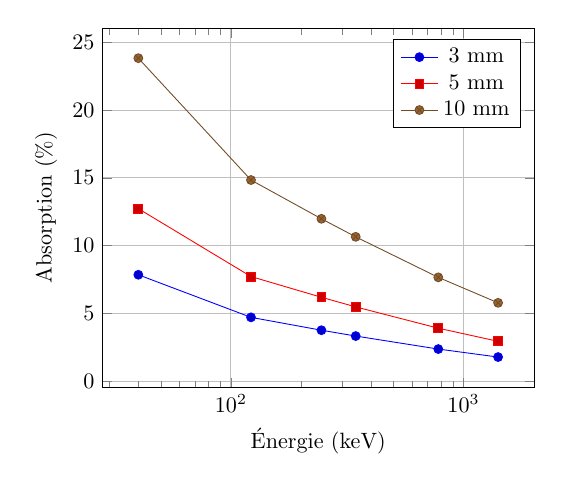
\begin{tikzpicture}[scale=0.8]
 \begin{axis}[
     xlabel={Énergie (keV)},
     ylabel={Absorption (\%)},
     legend pos=north east,
     grid=major,
     xmode=log,
 ]
 \addplot coordinates {(40,7.84) (122,4.70) (245,3.75) (344,3.32) (779,2.36) (1408,1.77)};
 \addplot coordinates {(40,12.72) (122,7.71) (245,6.18) (344,5.47) (779,3.90) (1408,2.93)};
 \addplot coordinates {(40,23.82) (122,14.83) (245,11.97) (344,10.64) (779,7.65) (1408,5.77)};
 \legend{3 mm, 5 mm, 10 mm}
 \end{axis}
 \end{tikzpicture}
 \captionsetup{labelformat=empty}
 \caption{\footnotesize Absorption des $\gamma$ Eu-152 en fonction de l'énergie et de l'épaisseur d'eau}
 \end{figure}

\clearpage

%==============================================================================
\normalsize
\noindent \begin{mdframed}[backgroundcolor=orange!20]
\section{\Large \color{blue} \textbf{Probabilite d'absorption par couche d'eau (1 cm) \\ Raies Eu-152 - Epaisseur totale : 3 cm}\color{black}}
\end{mdframed}
\footnotesize
%==============================================================================

\begin{tcolorbox}[colback=blue!5,colframe=blue!75!black,title=\textbf{Principe}]
\noindent Probabilite d'absorption par \color{blue}\textbf{couche d'eau}\color{black} \; pour les raies gamma de l'Eu-152
\end{tcolorbox}
\noindent Pour $\bm{N_0}$ photons incidents, apres traversee de $\bm{x}$ cm d'eau :
\begin{itemize}
\item Photons transmis : $\bm{N(x)} = \bm{N_0} \cdot e^{\bm{-\mu x}}$
\item Photons absorbes entre 0 et $\bm{x}$ : $\bm{N_0} \cdot \left[\bm{1} - e^{\bm{-\mu x}}\right]$
\end{itemize}
\noindent \color{blue}\textbf{Probabilite d'absorption dans la couche $\bm{n}$}\color{black} \; (de $(\bm{n-1})$ cm a $\bm{n}$ cm) :
\begin{equation*}
\bm{P}(\bm{\text{couche }} \bm{n}) = e^{-\bm{\mu }(\bm{n-1})} - e^{\bm{-\mu n}} = e^{\bm{-\mu} (\bm{n-1})} \cdot \left[\bm{1} - e^{\bm{-\mu}}\right]
\end{equation*}
\noindent \color{blue}\textbf{Verification :}\color{black}
\begin{equation*}
\bm{P(1)} + \bm{P(2)} + \bm{P(3)} = \bm{1} - e^{\bm{-3\mu}} = P(\bm{\text{total} sur \bm{3} cm})
\end{equation*}

\begin{table}[H]
\centering
\captionsetup{labelformat=empty}
\caption{Probabilite d'absorption par couche de 1 cm (epaisseur totale 3 cm)}
\begin{tabular}{@{}l c c c c c c c@{}}
\toprule
\footnotesize \textbf{Raie} &\footnotesize  \textbf{Energie} &\footnotesize  $\bm{\mu}$ &\footnotesize  \textbf{P(1er cm)} &\footnotesize  \textbf{P(2eme cm)} &\footnotesize  \textbf{P(3eme cm)} &\footnotesize  \textbf{P(total)} &\footnotesize  \textbf{Transmis} \\
 &\footnotesize  (keV) &\footnotesize  (cm$^{-1}$) &\footnotesize  (\%) &\footnotesize  (\%) &\footnotesize  (\%) &\footnotesize  (\%) &\footnotesize  (\%) \\
\midrule
\rowcolor{yellow!20}
\footnotesize 40 keV (X) &\footnotesize 39.52 &\footnotesize 0.272 &\footnotesize \textbf{23.82} &\footnotesize 18.15 &\footnotesize 13.82 &\footnotesize 55.80& \footnotesize 44.20 \\
\rowcolor{yellow!20}
\footnotesize 40 keV (X) &\footnotesize 40.12 &\footnotesize 0.268 &\footnotesize \textbf{23.49} &\footnotesize 17.97 &\footnotesize 13.75 &\footnotesize 55.21 &\footnotesize 44.79 \\
\footnotesize 122 keV &\footnotesize 121.78 &\footnotesize 0.161 &\footnotesize \textbf{14.83} &\footnotesize 12.63 &\footnotesize 10.76 &\footnotesize 38.23 &\footnotesize 61.77 \\
\footnotesize 245 keV &\footnotesize 244.70 &\footnotesize 0.128 &\footnotesize \textbf{11.97} &\footnotesize 10.54 &\footnotesize 9.28 &\footnotesize 31.79 &\footnotesize 68.21 \\
\rowcolor{yellow!20}
\footnotesize 344 keV &\footnotesize 344.28 &\footnotesize 0.112 &\footnotesize \textbf{10.64} &\footnotesize 9.50 &\footnotesize 8.49 &\footnotesize 28.63 &\footnotesize 71.37 \\
\footnotesize 411 keV &\footnotesize 411.12 &\footnotesize 0.105 &\footnotesize \textbf{9.96} &\footnotesize 8.97 &\footnotesize 8.07 &\footnotesize 27.00 &\footnotesize 73.00 \\
\footnotesize 444 keV &\footnotesize 443.96 &\footnotesize 0.102 &\footnotesize \textbf{9.67} &\footnotesize 8.73 &\footnotesize 7.89 &\footnotesize 26.29 &\footnotesize 73.71 \\
\footnotesize 779 keV &\footnotesize 778.90 &\footnotesize 0.080 &\footnotesize \textbf{7.65} &\footnotesize 7.07 &\footnotesize 6.53 & 21.24 &\footnotesize 78.76 \\
\footnotesize 867 keV &\footnotesize 867.38 &\footnotesize 0.076 &\footnotesize \textbf{7.29} &\footnotesize 6.76 &\footnotesize 6.26 &\footnotesize 20.31 &\footnotesize 79.69 \\
\footnotesize 964 keV &\footnotesize 964.08 &\footnotesize 0.072 &\footnotesize \textbf{6.94} &\footnotesize 6.46 &\footnotesize 6.01 &\footnotesize 19.42 &\footnotesize 80.58 \\
\footnotesize 1086 keV &\footnotesize 1085.84 &\footnotesize 0.068 &\footnotesize \textbf{6.56} &\footnotesize 6.13 &\footnotesize 5.73 &\footnotesize 18.42 &\footnotesize 81.58 \\
\footnotesize 1112 keV &\footnotesize 1112.07 &\footnotesize 0.067 &\footnotesize \textbf{6.49} &\footnotesize 6.06 &\footnotesize 5.67 &\footnotesize 18.22 &\footnotesize 81.78 \\
\rowcolor{yellow!20}
\footnotesize 1408 keV &\footnotesize 1408.01 &\footnotesize 0.060 &\footnotesize \textbf{5.77} &\footnotesize 5.44 &\footnotesize 5.13 &\footnotesize 16.34 &\footnotesize 83.66 \\
\bottomrule
\end{tabular}
\end{table}
\footnotesize
\noindent \textbf{Note :} Lignes surlignees = raies principales (intensite $> 20\%$)


%===============================================================================
\normalsize
\noindent \begin{mdframed}[backgroundcolor=orange!20]
\subsection{\color{blue}\textbf{Ratio entre couches successives}\color{black}}
\end{mdframed}
\footnotesize
%===============================================================================

\begin{table}[H]
\centering
\captionsetup{labelformat=empty}
\caption{\footnotesize Ratio d'absorption par couche (normalise au 1er cm)}
\begin{tabular}{@{}l c c c c c c@{}}
\toprule
\footnotesize \textbf{Raie} &\footnotesize \textbf{Energie} &\footnotesize \textbf{P(1er cm)} &\footnotesize \textbf{P(2eme cm)} &\footnotesize \textbf{P(3eme cm)} &\footnotesize \textbf{Ratio 2/1} &\footnotesize \textbf{Ratio 3/1} \\
 &\footnotesize (keV) &\footnotesize (\%) &\footnotesize (\%) &\footnotesize (\%) & & \\
\midrule
\footnotesize 40 keV (X) &\footnotesize 39.52 &\footnotesize 23.82 &\footnotesize 18.15 &\footnotesize 13.82 &\footnotesize 0.762 &\footnotesize 0.580 \\
\footnotesize 40 keV (X) &\footnotesize 40.12 &\footnotesize 23.49 &\footnotesize 17.97 &\footnotesize 13.75 &\footnotesize 0.765 &\footnotesize 0.585 \\
\footnotesize 122 keV &\footnotesize 121.78 &\footnotesize 14.83 &\footnotesize 12.63 &\footnotesize 10.76 &\footnotesize 0.852 &\footnotesize 0.725 \\
\footnotesize 245 keV &\footnotesize 244.70 &\footnotesize 11.97 &\footnotesize 10.54 &\footnotesize 9.28 &\footnotesize 0.880 &\footnotesize 0.775 \\
\footnotesize 344 keV &\footnotesize 344.28 &\footnotesize 10.64 &\footnotesize 9.50 &\footnotesize 8.49 &\footnotesize 0.894 &\footnotesize 0.799 \\
\footnotesize 411 keV &\footnotesize 411.12 &\footnotesize 9.96 &\footnotesize 8.97 &\footnotesize 8.07 &\footnotesize 0.900 &\footnotesize 0.811 \\
\footnotesize 444 keV &\footnotesize 443.96 &\footnotesize 9.67 &\footnotesize 8.73 &\footnotesize 7.89 &\footnotesize 0.903 &\footnotesize 0.816 \\
\footnotesize 779 keV &\footnotesize 778.90 &\footnotesize 7.65 &\footnotesize 7.07 &\footnotesize 6.53 &\footnotesize 0.923 &\footnotesize 0.853 \\
\footnotesize 867 keV &\footnotesize 867.38 &\footnotesize 7.29 &\footnotesize 6.76 &\footnotesize 6.26 &\footnotesize 0.927 &\footnotesize 0.860 \\
\footnotesize 964 keV &\footnotesize 964.08 &\footnotesize 6.94 &\footnotesize 6.46 &\footnotesize 6.01 &\footnotesize 0.931 &\footnotesize 0.866 \\
\footnotesize 1086 keV &\footnotesize 1085.84 &\footnotesize 6.56 &\footnotesize 6.13 &\footnotesize 5.73 &\footnotesize 0.934 &\footnotesize 0.873 \\
\footnotesize 1112 keV &\footnotesize 1112.07 &\footnotesize 6.49 &\footnotesize 6.06 &\footnotesize 5.67 &\footnotesize 0.935 &\footnotesize 0.875 \\
\footnotesize 1408 keV &\footnotesize 1408.01 &\footnotesize 5.77 &\footnotesize 5.44 &\footnotesize 5.13 &\footnotesize 0.942 &\footnotesize 0.888 \\
\bottomrule
\end{tabular}
\end{table}

\begin{table}[H]
\centering
\captionsetup{labelformat=empty}
\caption{\footnotesize Absorption moyenne ponderee par l'intensite des raies}
\begin{tabular}{@{}l c@{}}
\toprule
\footnotesize \textbf{Couche} &\footnotesize \textbf{Absorption} \\
\midrule
\footnotesize 1er cm (0--1 cm) &\footnotesize \textbf{13.48\%} \\
\footnotesize 2eme cm (1--2 cm) &\footnotesize \textbf{11.17\%} \\
\footnotesize 3eme cm (2--3 cm) &\footnotesize \textbf{9.32\%} \\
\midrule
\footnotesize \textbf{Total absorbe} &\footnotesize \textbf{33.98\%} \\
\footnotesize \textbf{Transmis} &\footnotesize \textbf{66.02\%} \\
\bottomrule
\end{tabular}
\end{table}


 %===============================================================================
\normalsize
\noindent \begin{mdframed}[backgroundcolor=orange!20]
\subsection{\color{blue}\textbf{Explication physique}\color{black}}
\end{mdframed}
\footnotesize
%===============================================================================
\medskip

\begin{tcolorbox}[colback=blue!5,colframe=blue!75!black,title=\textbf{Propriete fondamentale}]

\noindent Le ratio entre couches successives est \color{blue}\textbf{constant}\color{black} \; pour une energie donnee :

\begin{equation*}
\frac{P(\bm{\text{couche } n+1)}}{P(\bm{\text{couche } n)}} = e^{-\bm{\mu}}
\end{equation*}
\bm{}
\noindent Ce ratio represente la \color{blue}\textbf{fraction de photons qui survivent}\color{black} \;apres avoir traverse 1 cm d'eau.

\begin{itemize}
\item Plus $\bm{\mu}$ est grand (basse energie) $\rightarrow$ plus le ratio est petit (absorption rapide)
\item Plus $\bm{\mu}$ est petit (haute energie) $\rightarrow$ plus le ratio est proche de 1 (absorption uniforme)
\end{itemize}

\end{tcolorbox}

\begin{table}[H]
\centering
\captionsetup{labelformat=empty}
\caption{\footnotesize Interpretation physique du comportement d'absorption}
\begin{tabular}{@{}l c l@{}}
\toprule
\footnotesize \textbf{Energie} &\footnotesize $\bm{e^{-\mu}}$ &\footnotesize \textbf{Comportement} \\
\midrule
\footnotesize 40 keV &\footnotesize 0.76 &\footnotesize Absorption concentree dans le 1er cm \\
\footnotesize 122--444 keV &\footnotesize 0.85--0.90 &\footnotesize Decroissance moderee entre couches \\
\footnotesize 964--1408 keV &\footnotesize 0.93--0.94 &\footnotesize Absorption quasi-uniforme sur les 3 cm \\
\bottomrule
\end{tabular}
\end{table}

%===============================================================================
\normalsize
\noindent \begin{mdframed}[backgroundcolor=orange!20]
\subsection{\color{blue}\textbf{Synthese}\color{black}}
\end{mdframed}
\footnotesize
%===============================================================================
\medskip

\begin{tcolorbox}[colback=blue!5,colframe=blue!50!black,title=\textbf{Conclusions}]
\footnotesize 
\noindent \color{blue} \textbf{Pour les rayons X (40 keV) :}\color{black}
\begin{itemize}
\item Le 1er cm absorbe \color{blue}\textbf{24\%}\color{black} \; des photons
\item Le 2eme cm absorbe \color{blue}\textbf{18\%}\color{black} \; (seulement 76\% du 1er cm)
\item Le 3eme cm absorbe \color{blue}\textbf{14\%}\color{black} \; (seulement 58\% du 1er cm)
\item $\rightarrow$ L'absorption est \color{blue}\textbf{fortement concentree}\color{black} \; en surface
\end{itemize}

\vspace{0.1cm}

\noindent \color{blue}\textbf{Pour les gammas de haute energie (1408 keV) :}\color{black}

\begin{itemize}
\item Le 1er cm absorbe \color{blue}\textbf{5.8\%}\color{black} des photons
\item Le 2eme cm absorbe \color{blue}\textbf{5.4\%}\color{black}  \;(94\% du 1er cm)
\item Le 3eme cm absorbe \color{blue}\textbf{5.1\%}\color{black}  \;(89\% du 1er cm)
\item $\rightarrow$ L'absorption est \color{blue}\textbf{quasi-uniforme}\color{black}  \;en profondeur
\end{itemize}

\vspace{0.1cm}

\noindent \color{blue}\textbf{Moyenne ponderee (toutes raies) :}\color{black}
\begin{center}
\begin{tabular}{ccc}
\footnotesize \textbf{1er cm} &\footnotesize \textbf{2eme cm} &\footnotesize \textbf{3eme cm} \\
\footnotesize 13.5\% &\footnotesize 11.2\% &\footnotesize 9.3\% \\
\end{tabular}
\end{center}

\noindent Apres 3 cm d'eau, \color{blue}\textbf{34\%}\color{black} \; des gammas de l'Eu-152 sont absorbes et \color{blue}\textbf{66\%}\color{black} \; sont transmis.

\end{tcolorbox}

\clearpage

%==============================================================================
\normalsize
\noindent \begin{mdframed}[backgroundcolor=orange!20]
\section{\Large \color{blue} \textbf{Probabilite d'absorption par couche d'eau (5 mm) \\ Raies Eu-152 - Epaisseur totale : 15 mm}\color{black}}
\end{mdframed}
\footnotesize
%==============================================================================

\begin{table}[H]
\centering
\captionsetup{labelformat=empty}
\caption{\footnotesize Probabilite d'absorption par couche de 5 mm (epaisseur totale 15 mm)}
\begin{tabular}{@{}l c c c c c c c@{}}
\toprule
\footnotesize\textbf{Raie} &\footnotesize \textbf{Energie} &\footnotesize $\bm{\mu}$ &\footnotesize \textbf{P(1er 5mm)} &\footnotesize \textbf{P(2eme 5mm)} &\footnotesize \textbf{P(3eme 5mm)} &\footnotesize \textbf{P(total)} &\footnotesize \textbf{Transmis} \\
 &\footnotesize (keV) &\footnotesize (cm$^{-1}$) &\footnotesize (\%) &\footnotesize (\%) &\footnotesize (\%) &\footnotesize (\%) &\footnotesize (\%) \\
\midrule
\rowcolor{yellow!20}
\footnotesize 40 keV (X) &\footnotesize 39.52 &\footnotesize 0.272 &\footnotesize \textbf{12.72} &\footnotesize 11.10 &\footnotesize 9.69 &\footnotesize 33.51 &\footnotesize 66.49 \\
\rowcolor{yellow!20}
\footnotesize 40 keV (X) &\footnotesize 40.12 &\footnotesize 0.268 &\footnotesize \textbf{12.53} &\footnotesize 10.96 &\footnotesize 9.\footnotesize 59 &\footnotesize 33.07 &\footnotesize 66.93 \\
\footnotesize 122 keV &\footnotesize 121.78 &\footnotesize 0.161 &\footnotesize \textbf{7.71} &\footnotesize 7.12 & 6.57 & 21.40 & 78.60 \\
\footnotesize 245 keV &\footnotesize 244.70 &\footnotesize 0.128 &\footnotesize \textbf{6.18} &\footnotesize 5.80 &\footnotesize 5.44 &\footnotesize 17.41 &\footnotesize 82.59 \\
\rowcolor{yellow!20}
\footnotesize 344 keV &\footnotesize 344.28 &\footnotesize 0.112 &\footnotesize \textbf{5.47} &\footnotesize 5.17 &\footnotesize 4.89 &\footnotesize 15.52 &\footnotesize 84.48 \\
\footnotesize 411 keV &\footnotesize 411.12 &\footnotesize 0.105 &\footnotesize \textbf{5.11} &\footnotesize 4.85 &\footnotesize 4.60 &\footnotesize 14.56 &\footnotesize 85.44 \\
\footnotesize 444 keV &\footnotesize 443.96 &\footnotesize 0.102 &\footnotesize \textbf{4.96} &\footnotesize 4.71 &\footnotesize 4.48 &\footnotesize 14.15 &\footnotesize 85.85 \\
\footnotesize 779 keV &\footnotesize 778.90 &\footnotesize 0.080 &\footnotesize \textbf{3.90} &\footnotesize 3.75 &\footnotesize 3.60 &\footnotesize 11.26 &\footnotesize 88.74 \\
\footnotesize 867 keV &\footnotesize 867.38 &\footnotesize 0.076 &\footnotesize \textbf{3.71} &\footnotesize 3.58 &\footnotesize 3.44 & \footnotesize 10.73 &\footnotesize 89.27 \\
\footnotesize 964 keV &\footnotesize 964.08 &\footnotesize 0.072 &\footnotesize \textbf{3.53} &\footnotesize 3.41 &\footnotesize 3.29 & 10.23 &\footnotesize 89.77 \\
\footnotesize 1086 keV &\footnotesize 1085.84 &\footnotesize 0.068 &\footnotesize \textbf{3.34} &\footnotesize 3.22 &\footnotesize 3.12 &\footnotesize 9.68 &\footnotesize 90.32 \\
\footnotesize 1112 keV &\footnotesize 1112.07 &\footnotesize 0.067 &\footnotesize \textbf{3.30} &\footnotesize 3.19 &\footnotesize 3.08 &\footnotesize 9.57 &\footnotesize 90.43 \\
\rowcolor{yellow!20}
\footnotesize1408 keV &\footnotesize 1408.01 &\footnotesize 0.060 &\footnotesize \textbf{2.93} &\footnotesize 2.84 &\footnotesize 2.76 &\footnotesize 8.53 &\footnotesize 91.47 \\
\bottomrule
\end{tabular}

\vspace{0.1cm}
\footnotesize
\textbf{Note :} Lignes surlignees = raies principales (intensite $> 20\%$)
\end{table}

\begin{table}[H]
\centering
\captionsetup{labelformat=empty}
\caption{\footnotesize Absorption moyenne ponderee par l'intensite des raies}
\begin{tabular}{@{}l c@{}}
\toprule
\footnotesize \textbf{Couche} &\footnotesize \textbf{Absorption} \\
\midrule
\footnotesize 1er 5mm (0--5 mm) &\footnotesize \textbf{7.06\%} \\
\footnotesize 2eme 5mm (5--10 mm) &\footnotesize \textbf{6.42\%} \\
\footnotesize 3eme 5mm (10--15 mm) &\footnotesize \textbf{5.84\%} \\
\midrule
\footnotesize \textbf{Total absorbe} &\footnotesize \textbf{19.33\%} \\
\footnotesize \textbf{Transmis} &\footnotesize \textbf{80.67\%} \\
\bottomrule
\end{tabular}
\end{table}

%===============================================================================
\normalsize
\noindent \begin{mdframed}[backgroundcolor=orange!20]
\subsection{\color{blue}\textbf{Ratio entre couches successives}\color{black}}
\end{mdframed}
\footnotesize
%===============================================================================
\medskip

\begin{table}[H]
\centering
\captionsetup{labelformat=empty}
\caption{\footnotesize Ratio d'absorption par couche (normalise au 1er 5mm)}
\begin{tabular}{@{}l c c c c c c@{}}
\toprule
\footnotesize \textbf{Raie} &\footnotesize \textbf{Energie} &\footnotesize \textbf{P(1er 5mm)} &\footnotesize \textbf{P(2eme 5mm)} &\footnotesize \textbf{P(3eme 5mm)} &\footnotesize \textbf{Ratio 2/1} &\footnotesize \textbf{Ratio 3/1} \\
 &\footnotesize (keV) &\footnotesize (\%) &\footnotesize (\%) &\footnotesize (\%) & & \\
\midrule
\footnotesize 40 keV (X) &\footnotesize 39.52 &\footnotesize 12.72 &\footnotesize 11.10 &\footnotesize 9.69 &\footnotesize 0.873 &\footnotesize 0.762 \\
\footnotesize 40 keV (X) &\footnotesize 40.12 &\footnotesize 12.53 &\footnotesize 10.96 &\footnotesize 9.59 &\footnotesize 0.875 &\footnotesize 0.765 \\
\footnotesize 122 keV &\footnotesize 121.78 &\footnotesize 7.71 &\footnotesize 7.12 &\footnotesize 6.57 &\footnotesize 0.923 &\footnotesize 0.852 \\
\footnotesize 245 keV &\footnotesize 244.70 &\footnotesize 6.18 &\footnotesize 5.80 &\footnotesize 5.44 &\footnotesize 0.938 &\footnotesize 0.880 \\
\footnotesize 344 keV &\footnotesize 344.28 &\footnotesize 5.47 &\footnotesize 5.17 &\footnotesize 4.89 &\footnotesize 0.945 &\footnotesize 0.894 \\
\footnotesize 411 keV &\footnotesize 411.12 &\footnotesize 5.11 &\footnotesize 4.85 &\footnotesize 4.60 &\footnotesize 0.949 &\footnotesize 0.900 \\
\footnotesize 444 keV &\footnotesize 443.96 &\footnotesize 4.96 &\footnotesize 4.71 &\footnotesize 4.48 &\footnotesize 0.950 &\footnotesize 0.903 \\
\footnotesize 779 keV &\footnotesize 778.90 &\footnotesize 3.90 &\footnotesize 3.75 &\footnotesize 3.60 &\footnotesize 0.961 &\footnotesize 0.923 \\
\footnotesize 867 keV &\footnotesize 867.38 &\footnotesize 3.71 &\footnotesize 3.58 &\footnotesize 3.44 &\footnotesize 0.963 &\footnotesize 0.927 \\
\footnotesize 964 keV &\footnotesize 964.08 &\footnotesize 3.53 &\footnotesize 3.41 &\footnotesize 3.29 &\footnotesize 0.965 &\footnotesize 0.931 \\
\footnotesize 1086 keV &\footnotesize 1085.84 &\footnotesize 3.34 &\footnotesize 3.22 &\footnotesize 3.12 &\footnotesize 0.967 &\footnotesize 0.934 \\
\footnotesize 1112 keV &\footnotesize 1112.07 &\footnotesize 3.30 &\footnotesize 3.19 &\footnotesize 3.08 &\footnotesize 0.967 &\footnotesize 0.935 \\
\footnotesize 1408 keV &\footnotesize 1408.01 &\footnotesize 2.93 &\footnotesize 2.84 &\footnotesize 2.76 &\footnotesize 0.971 &\footnotesize 0.942 \\
\bottomrule
\end{tabular}
\end{table}

 %===============================================================================
\normalsize
\noindent \begin{mdframed}[backgroundcolor=orange!20]
\subsection{\color{blue}\textbf{Explication physique}\color{black}}
\end{mdframed}
\footnotesize
%===============================================================================
\medskip

\begin{tcolorbox}[colback=blue!5,colframe=blue!75!black,title=\textbf{Propriete fondamentale}]

\noindent Le ratio entre couches successives est \color{blue}\textbf{constant}\color{black} \; pour une energie donnee :

\begin{equation}
\frac{\bm{P}(\bm{\text{couche }} \bm{n+1})}{\bm{P}(\bm{\text{couche }} \bm{n})} = e^{-\bm{0.5\mu}}
\end{equation}

\noindent Ce ratio represente la \color{blue}\textbf{fraction de photons qui survivent}\color{black} \; apres avoir traverse 5 mm d'eau.

\begin{itemize}
\item Plus $\bm{\mu}$ est grand (basse energie) $\rightarrow$ plus le ratio est petit (absorption plus rapide)
\item Plus $\bm{\mu}$ est petit (haute energie) $\rightarrow$ plus le ratio est proche de 1 (absorption uniforme)
\end{itemize}

\end{tcolorbox}

\begin{table}[H]
\centering
\captionsetup{labelformat=empty}
\caption{\footnotesize Interpretation physique du comportement d'absorption}
\begin{tabular}{@{}l c l@{}}
\toprule
\footnotesize \textbf{Energie} &\footnotesize $\bm{e^{-0.5\mu}}$ &\footnotesize \textbf{Comportement} \\
\midrule
\footnotesize 40 keV &\footnotesize  0.87 &\footnotesize  Absorption plus forte dans le 1er 5mm \\
\footnotesize --444 keV &\footnotesize 0.92--0.95 &\footnotesize Decroissance moderee entre couches \\
\footnotesize 779--1408 keV &\footnotesize 0.96--0.97 &\footnotesize Absorption quasi-uniforme sur les 15 mm \\
\bottomrule
\end{tabular}
\end{table}

%===============================================================================
\normalsize
\noindent \begin{mdframed}[backgroundcolor=orange!20]
\subsection{\color{blue}\textbf{Synthese}\color{black}}
\end{mdframed}
\footnotesize
%===============================================================================
\medskip

\begin{tcolorbox}[colback=blue!5,colframe=blue!50!black,title=\textbf{Conclusions}]

\textbf{Pour les rayons X (40 keV) :}
\begin{itemize}
\item Le 1er 5mm absorbe \color{blue}\textbf{12.7\%}\color{black} \; des photons
\item Le 2eme 5mm absorbe \color{blue}\textbf{11.1\%}\color{black} \; (87\% du 1er)
\item Le 3eme 5mm absorbe \color{blue}\textbf{9.7\%}\color{black} \; (76\% du 1er)
\item $\rightarrow$ L'absorption est \textbf{legerement concentree} en surface
\end{itemize}

\vspace{0.1cm}

\textbf{Pour les gammas de haute energie (1408 keV) :}
\begin{itemize}
\item Le 1er 5mm absorbe \color{blue}\textbf{2.93\%}\color{black} \; des photons
\item Le 2eme 5mm absorbe \color{blue}\textbf{2.84\%}\color{black} \; (97\% du 1er)
\item Le 3eme 5mm absorbe \color{blue}\textbf{2.76\%}\color{black} \; (94\% du 1er)
\item $\rightarrow$ L'absorption est \color{blue}\textbf{quasi-uniforme}\color{black} \; en profondeur
\end{itemize}

\vspace{0.1cm}

\noindent \textbf{Moyenne ponderee (toutes raies) :}
\begin{center}
\begin{tabular}{ccc}
\footnotesize \textbf{1er 5mm} &\footnotesize \textbf{2eme 5mm} &\footnotesize \textbf{3eme 5mm} \\
\footnotesize 7.06\% &\footnotesize 6.42\% &\footnotesize 5.84\% \\
\end{tabular}
\end{center}

\noindent Apres 15 mm d'eau, \color{blue}\textbf{19.3\%}\color{black} \; des gammas de l'Eu-152 sont absorbes et \color{blue}\textbf{80.7\%}\color{black} \; sont transmis.

\end{tcolorbox}

%===============================================================================
\normalsize
\noindent \begin{mdframed}[backgroundcolor=orange!20]
\subsection{\color{blue}\textbf{Comparaison avec les couches de 1 cm}\color{black}}
\end{mdframed}
\footnotesize
%===============================================================================
\medskip

\begin{table}[H]
\centering
\captionsetup{labelformat=empty}
\caption{\footnotesize comparaison des absorptions moyennes ponderees}
\begin{tabular}{@{}l c c@{}}
\toprule
\footnotesize \textbf{Configuration} &\footnotesize \textbf{Epaisseur totale} &\footnotesize \textbf{Absorption totale} \\
\midrule
\footnotesize 3 couches de 5 mm &\footnotesize 15 mm &\footnotesize 19.3\% \\
\footnotesize 3 couches de 10 mm &\footnotesize 30 mm &\footnotesize 34.0\% \\
\bottomrule
\end{tabular}
\end{table}

\clearpage


%==============================================================================
\normalsize
\noindent \begin{mdframed}[backgroundcolor=orange!20]
\section{\Large \color{blue} \textbf{Probabilite d'absorption par couche d'eau (5 mm) \\ Raies Eu-152 - Comparaison : 1er 5mm vs (2eme + 3eme) 5mm}\color{black}}
\end{mdframed}
\footnotesize
%==============================================================================

\begin{tcolorbox}[colback=blue!5,colframe=blue!75!black,title=\textbf{Configuration}]
\begin{itemize}
\item \color{blue}\textbf{Epaisseur totale :}\color{black} \; 15 mm (1.5 cm)
\item \color{blue}\textbf{Couche 1 :}\color{black} \; 0--5 mm (5 mm)
\item \color{blue}\textbf{Couches 2+3 :}\color{black} \; 5--15 mm (10 mm)
\end{itemize}
\end{tcolorbox}

\begin{tcolorbox}[colback=blue!5,colframe=blue!75!black,title=\textbf{Probabilites d'absorption}]

\noindent \color{blue}\textbf{1er 5mm (0--5 mm) :}\color{black}
\begin{equation*}
\bm{P_1} = \bm{1} - e^{\bm{-0.5\mu}}
\end{equation*}
\noindent \color{blue}\textbf{2eme + 3eme 5mm (5--15 mm) :}\color{black}
\begin{equation*}
\bm{P_{2+3}} = e^{\bm{-0.5\mu}} - e^{\bm{-1.5\mu}}
\end{equation*}
\noindent  \color{blue}\textbf{Ratio :}\color{black}
\begin{equation*}
\bm{\text{Ratio}} = \frac{\bm{P_{2+3}}}{\bm{P_1}} = \frac{e^{\bm{-0.5\mu}} - e^{\bm{-1.5\mu}}}{\bm{1} - e^{\bm{-0.5\mu}}}
\end{equation*}
\end{tcolorbox}

\begin{table}[H]
\centering
\captionsetup{labelformat=empty}
\caption{\footnotesize Probabilite d'absorption : 1er 5mm vs (2eme + 3eme) 5mm}
\begin{tabular}{@{}l c c c c c c c@{}}
\toprule
\footnotesize \textbf{Raie} &\footnotesize  \textbf{Energie} &\footnotesize  $\bm{\mu}$ &\footnotesize  \textbf{P(1er 5mm)} &\footnotesize  \textbf{P(2+3 5mm)} &\footnotesize  \textbf{P(total)} &\footnotesize  \textbf{Ratio} &\footnotesize  \textbf{Transmis} \\
 &\footnotesize  (keV) &\footnotesize  (cm$^{-1}$) &\footnotesize  0--5 mm &\footnotesize  5--15 mm &\footnotesize  0--15 mm &\footnotesize  (2+3)/1 &\footnotesize  (\%) \\
\midrule
\rowcolor{yellow!20}
\footnotesize 40 keV (X) &\footnotesize  39.52 &\footnotesize  0.272 &\footnotesize  \textbf{12.72\%} &\footnotesize 20.79\% &\footnotesize 33.51\% &\footnotesize 1.635 &\footnotesize 66.49 \\
\rowcolor{yellow!20}
\footnotesize 40 keV (X) &\footnotesize 40.12&\footnotesize 0.268&\footnotesize \textbf{12.53\%}&\footnotesize \textbf{20.54\%}&\footnotesize 33.07\% &\footnotesize 1.640 &\footnotesize  66.93 \\
\footnotesize 122 keV &\footnotesize  121.78 &\footnotesize 0.161&\footnotesize \textbf{7.71\%}&\footnotesize \textbf{13.69\%}&\footnotesize 21.40\% &\footnotesize 1.775 &\footnotesize 78.60 \\
\footnotesize 245 keV&\footnotesize 244.70&\footnotesize 0.128&\footnotesize  \textbf{6.18\%}&\footnotesize \textbf{11.23\%} &\footnotesize 17.41\% &\footnotesize 1.819 &\footnotesize  82.59 \\
\rowcolor{yellow!20}
\footnotesize 344 keV&\footnotesize 344.28&\footnotesize 0.112&\footnotesize \textbf{5.47\%}&\footnotesize \textbf{10.05\%}&\footnotesize 15.52\% &\footnotesize 1.839&\footnotesize 84.48 \\
\footnotesize 411 keV&\footnotesize 411.12&\footnotesize 0.105&\footnotesize \textbf{5.11\%}&\footnotesize \textbf{9.45\%}&\footnotesize 14.56\% &\footnotesize 1.849&\footnotesize 85.44 \\
\footnotesize 444 keV&\footnotesize 443.96&\footnotesize 0.102&\footnotesize \textbf{4.96\%}&\footnotesize \textbf{9.19\%}&\footnotesize 14.15\% &\footnotesize 1.854&\footnotesize  85.85 \\
\footnotesize 779 keV&\footnotesize 778.90&\footnotesize 0.080&\footnotesize \textbf{3.90\%}&\footnotesize \textbf{7.35\%}&\footnotesize 11.26\% &\footnotesize 1.884 &\footnotesize 88.74 \\
\footnotesize 867 keV&\footnotesize 867.38&\footnotesize 0.076&\footnotesize \textbf{3.71\%}&\footnotesize \textbf{7.02\%}&\footnotesize 10.73\% &\footnotesize 1.890 &\footnotesize 89.27 \\
\footnotesize 964 keV&\footnotesize 964.08&\footnotesize 0.072&\footnotesize \textbf{3.53\%}&\footnotesize \textbf{6.70\%}&\footnotesize 10.23\% &\footnotesize 1.895&\footnotesize  89.77 \\
\footnotesize 1086 keV&\footnotesize 1085.84&\footnotesize 0.068&\footnotesize \textbf{3.34\%}&\footnotesize \textbf{6.34\%}&\footnotesize 9.68\% &\footnotesize 1.901&\footnotesize 90.32 \\
\footnotesize 1112 keV&\footnotesize 1112.07&\footnotesize 0.067&\footnotesize \textbf{3.30\%}&\footnotesize \textbf{6.27\%}&\footnotesize 9.57\% &\footnotesize 1.902&\footnotesize 90.43 \\
\rowcolor{yellow!20}
\footnotesize 1408 keV&\footnotesize 1408.01&\footnotesize 0.060&\footnotesize \textbf{2.93\%}&\footnotesize \textbf{5.60\%}&\footnotesize 8.53\% &\footnotesize 1.913 &\footnotesize  91.47 \\
\bottomrule
\end{tabular}
\end{table}
\vspace{0.1cm}
\footnotesize
\noindent \textbf{Note :} Lignes surlignees = raies principales (intensite $> 20\%$)



\normalsize
\noindent \begin{mdframed}[backgroundcolor=orange!20]
\subsection{\color{blue}\textbf{Interpretation physique}\color{black}}
\end{mdframed}
\footnotesize
\medskip

\begin{tcolorbox}[colback=blue!5,colframe=blue!50!black,title=\textbf{Signification du ratio (2+3)/1}]

\noindent Le ratio $\displaystyle\frac{\bm{P_{2+3}}}{\bm{P_1}}$ compare l'absorption dans les 10 mm suivants (5--15 mm) a celle dans les 5 premiers mm (0--5 mm).

\vspace{0.1cm}

\begin{tabular}{@{}l l@{}}
\footnotesize $\bullet$ Ratio $< 1$ : &\footnotesize Plus d'absorption dans le 1er 5mm que dans les 10 mm suivants \\
\footnotesize $\bullet$ Ratio $= 1$ : &\footnotesize Absorption egale (surface = profondeur $\times$ 2) \\
\footnotesize $\bullet$ Ratio $= 2$ : &\footnotesize Absorption uniforme (2$\times$ l'epaisseur $\rightarrow$ 2$\times$ l'absorption) \\
\footnotesize $\bullet$ Ratio $> 2$ : &\footnotesize Plus d'absorption en profondeur qu'en surface \\
\end{tabular}

\end{tcolorbox}

\begin{table}[H]
\centering
\captionsetup{labelformat=empty}
\caption{\footnotesize Variation du ratio selon l'energie}
\begin{tabular}{@{}l c l@{}}
\toprule
\footnotesize \textbf{Energie} &\footnotesize \textbf{Ratio (2+3)/1} &\footnotesize \textbf{Interpretation} \\
\midrule
\footnotesize 40 keV (X-rays) &\footnotesize 1.64 &\footnotesize Absorption decroit en profondeur \\
\footnotesize 122--444 keV &\footnotesize 1.78--1.85 &\footnotesize Decroissance moderee \\
\footnotesize 779--1408 keV &\footnotesize 1.88--1.91 &\footnotesize Proche de l'absorption uniforme \\
\midrule
\footnotesize \textbf{Moyenne ponderee} &\footnotesize \textbf{1.74} & \\
\bottomrule
\end{tabular}
\end{table}

\begin{table}[H]
\centering
\captionsetup{labelformat=empty}
\caption{\footnotesize Absorption moyenne ponderee par l'intensite des raies}
\begin{tabular}{@{}l c@{}}
\toprule
\footnotesize \textbf{Zone} &\footnotesize \textbf{Absorption} \\
\midrule
\footnotesize 1er 5mm (0--5 mm) &\footnotesize \textbf{7.06\%} \\
\footnotesize 2eme+3eme 5mm (5--15 mm) &\footnotesize \textbf{12.26\%} \\
\midrule
\footnotesize \textbf{Total absorbe} &\footnotesize \textbf{19.33\%} \\
\footnotesize \textbf{Transmis} &\footnotesize \textbf{80.67\%} \\
\midrule
\footnotesize \textbf{Ratio (2+3)/1} &\footnotesize \textbf{1.74} \\
\bottomrule
\end{tabular}
\end{table}

\normalsize
\noindent \begin{mdframed}[backgroundcolor=orange!20]
\subsection{\color{blue}\textbf{Synthese}\color{black}}
\end{mdframed}
\footnotesize
\medskip

\begin{tcolorbox}[colback=blue!5,colframe=blue!75!black,title=\textbf{Conclusions}]

\noindent \color{blue}\textbf{Repartition de l'absorption dans 15 mm d'eau :}\color{black}

\begin{center}
\begin{tabular}{|c|c|c|}
\hline
\rowcolor{blue!20}
\footnotesize \textbf{1er 5mm} &\footnotesize \textbf{2eme+3eme 5mm} &\footnotesize \textbf{Total} \\
\footnotesize \textbf{(0--5 mm)} &\footnotesize \textbf{(5--15 mm)} &\footnotesize \textbf{(0--15 mm)} \\
\hline
\footnotesize 7.06\% &\footnotesize  12.26\% &\footnotesize 19.33\% \\
\hline
\footnotesize \textit{36.5\% du total} &\footnotesize \textit{63.5\% du total} &\footnotesize 100\% \\
\hline
\end{tabular}
\end{center}

\vspace{0.1cm}

\noindent \color{blue}\textbf{Observations :}\color{black}
\begin{itemize}
\item Le ratio moyen de \color{blue}\textbf{1.74} est inferieur a 2, ce qui traduit l'attenuation exponentielle du faisceau.
\item Pour les basses energies (40 keV), le ratio est plus faible (\color{blue}\textbf{1.64}\color{black}) car l'absorption decroit plus rapidement avec la profondeur.
\item Pour les hautes energies (1408 keV), le ratio tend vers 2 (\color{blue}\textbf{1.91}\color{black}) car l'absorption est quasi-uniforme.
\item En moyenne, les 10 mm de profondeur absorbent \color{blue}\textbf{1.74$\times$}\color{black} \; plus que les 5 premiers mm (au lieu de 2$\times$ si l'absorption etait parfaitement uniforme).
\end{itemize}

\end{tcolorbox}

\normalsize
\noindent \begin{mdframed}[backgroundcolor=orange!20]
\subsection{\color{blue}\textbf{Formule generale du ratio}\color{black}}
\end{mdframed}
\footnotesize
\medskip

\noindent Pour une couche d'epaisseur $\bm{d}$ suivie d'une couche d'epaisseur $\bm{2d}$ :

\begin{equation*}
\bm{\text{Ratio}} = \frac{\bm{P}(\bm{d} \to \bm{3d})}{\bm{P}(\bm{0} \to \bm{d})} = \frac{e^{\bm{-\mu d}} - e^{\bm{-3\mu d}}}{\bm{1} - e^{\bm{-\mu d}}} = \frac{e^{\bm{-\mu d}}(\bm{1} - e^{\bm{-2\mu d}})}{\bm{1} - e^{\bm{-\mu d}}}
\end{equation*}

\noindent \color{blue}\textbf{Cas limites :}\color{black}

\begin{itemize}
\item Si $\bm{\mu d} \to 0$ (faible absorption) : Ratio $\to 2$ (absorption uniforme)
\item Si $\bm{\mu d} \to \infty$ (forte absorption) : Ratio $\to 0$ (tout absorbe dans la 1ere couche)
\end{itemize}

\clearpage


%==============================================================================
\normalsize
\noindent \begin{mdframed}[backgroundcolor=orange!20]
\section{\Large \color{blue} \textbf{Probabilite d'absorption dans 1 cm d'eau \\ Distribution uniforme 0-50 keV - 10 bins de 5 keV chacun}\color{black}}
\end{mdframed}
\footnotesize
%==============================================================================


\begin{tcolorbox}[colback=blue!5,colframe=blue!75!black,title=\textbf{Probabilite d'absorption}]

\noindent \color{blue} \textbf{Probabilite d'absorption dans 1 cm d'eau :}\color{black}

\begin{equation*}
\bm{P}(\bm{1}\,\text{cm}) = \bm{1} - e^{\bm{-\mu} \times \bm{1}\,\text{cm}} = \bm{1} - e^{\bm{-\mu}}
\end{equation*}

\noindent avec $\bm{\mu} = \bm{\mu}/\bm{\rho} \times \bm{\rho_{\text{eau}}} = \bm{\mu}/\bm{\rho} \times \bm{1}\,\text{g/cm}^3 = \bm{\mu}/\bm{\rho}$ (en cm$^{-1}$)

\end{tcolorbox}

\begin{table}[H]
\centering
\captionsetup{labelformat=empty}
\caption{\footnotesize Probabilite d'absorption dans 1 cm d'eau -- Distribution uniforme 0--50 keV}
\begin{tabular}{@{}c c c c c c@{}}
\toprule
\footnotesize \textbf{Bin}&\footnotesize \textbf{Plage}&\footnotesize \textbf{E$_{\text{centre}}$}&\footnotesize $\bm{\mu}$&\footnotesize \textbf{P(1 cm)}&\footnotesize \textbf{Transmis} \\
 &\footnotesize (keV)&\footnotesize (keV)&\footnotesize (cm$^{-1}$)&\footnotesize (\%)&\footnotesize (\%) \\
\midrule
\rowcolor{red!20}
\footnotesize 1&\footnotesize 0--5&\footnotesize 2.5&\footnotesize 325.6&\footnotesize $\sim$\textbf{100}&\footnotesize $\sim$0 \\
\rowcolor{red!20}
\footnotesize 2&\footnotesize 5--10&\footnotesize 7.5&\footnotesize 12.07&\footnotesize $\sim$\textbf{100}&\footnotesize $\sim$0 \\
\rowcolor{orange!20}
\footnotesize 3&\footnotesize 10--15&\footnotesize 12.5&\footnotesize 2.82&\footnotesize \textbf{94.0}&\footnotesize 6.0 \\
\rowcolor{orange!20}
\footnotesize 4&\footnotesize 15--20&\footnotesize 17.5&\footnotesize 1.13&\footnotesize \textbf{67.8}&\footnotesize 32.2 \\
\rowcolor{yellow!20}
\footnotesize 5&\footnotesize 20--25&\footnotesize 22.5&\footnotesize 0.65&\footnotesize \textbf{47.7}&\footnotesize 52.3 \\
\rowcolor{yellow!20}
\footnotesize 6&\footnotesize 25--30&\footnotesize 27.5&\footnotesize 0.44&\footnotesize \textbf{35.8}&\footnotesize 64.2 \\
\rowcolor{yellow!20}
\footnotesize 7&\footnotesize 30--35&\footnotesize 32.5&\footnotesize 0.34&\footnotesize \textbf{29.0}&\footnotesize 71.0 \\
\rowcolor{green!20}
\footnotesize 8&\footnotesize 35--40 &\footnotesize 37.5&\footnotesize 0.29&\footnotesize \textbf{25.1}&\footnotesize 74.9 \\
\rowcolor{green!20}
\footnotesize 9&\footnotesize 40--45 &\footnotesize 42.5&\footnotesize 0.26&\footnotesize \textbf{22.6}&\footnotesize 77.4 \\
\rowcolor{green!20}
\footnotesize 10&\footnotesize 45--50 &\footnotesize 47.5&\footnotesize 0.24&\footnotesize \textbf{21.0}&\footnotesize 79.0 \\
\bottomrule
\end{tabular}
\end{table}
\vspace{0.1cm}
\footnotesize
\noindent \textbf{Code couleur :} \\
\noindent \colorbox{red!20}{Absorption totale}   \\
\noindent \colorbox{orange!20}{Absorption forte}  \\
\noindent \colorbox{yellow!20}{Absorption partielle} \\
\noindent \colorbox{green!20}{Transmission significative}\\

\begin{table}[H]
\centering
\captionsetup{labelformat=empty}
\caption{\footnotesize Absorption moyenne pour une distribution uniforme 0--50 keV}
\begin{tabular}{@{}l c@{}}
\toprule
\footnotesize \textbf{Grandeur} &\footnotesize \textbf{Valeur} \\
\midrule
\footnotesize Absorption moyenne dans 1 cm d'eau &\footnotesize \textbf{54.3\%} \\
\footnotesize Transmission moyenne apres 1 cm &\footnotesize \textbf{45.7\%} \\
\bottomrule
\end{tabular}
\end{table}

\begin{table}[H]
\centering
\captionsetup{labelformat=empty}
\caption{\footnotesize Absorption par gamme d'energie}
\begin{tabular}{@{}l c c l@{}}
\toprule
\footnotesize \textbf{Categorie} &\footnotesize \textbf{Energie} &\footnotesize \textbf{P(1 cm)} &\footnotesize \textbf{Commentaire} \\
\midrule
\rowcolor{red!20}
\footnotesize Tres basse energie &\footnotesize 0--10 keV &\footnotesize $\sim$100\% &\footnotesize Absorption totale \\
\rowcolor{orange!20}
\footnotesize Basse energie &\footnotesize 10--20 keV &\footnotesize $\sim$81\% &\footnotesize Absorption quasi-totale \\
\rowcolor{yellow!20}
\footnotesize Moyenne energie &\footnotesize 20--35 keV &\footnotesize $\sim$37\% &\footnotesize Absorption partielle \\
\rowcolor{green!20}
\footnotesize Haute energie &\footnotesize 35--50 keV &\footnotesize $\sim$23\% &\footnotesize Transmission significative \\
\bottomrule
\end{tabular}
\end{table}

\begin{tcolorbox}[colback=blue!5,colframe=blue!75!black,title=\textbf{Comparaison avec les gammas Eu-152}]

\begin{center}
\begin{tabular}{@{}l c | l c@{}}
\toprule
\multicolumn{2}{c|}{\footnotesize\textbf{Distribution 0--50 keV}}&\multicolumn{2}{c}{\footnotesize \textbf{Eu-152}} \\
\footnotesize \textbf{Energie}&\footnotesize \textbf{P(1 cm)}&\footnotesize \textbf{Energie}&\footnotesize \textbf{P(1 cm)} \\
\midrule
\footnotesize 2.5 keV &\footnotesize $\sim$100\% &\footnotesize 4 0 keV (X) &\footnotesize 23.8\% \\
\footnotesize 12.5 keV &\footnotesize 94.0\% &\footnotesize 122 keV &\footnotesize 14.8\% \\
\footnotesize 27.5 keV &\footnotesize 35.8\% &\footnotesize 344 keV &\footnotesize 10.6\% \\
\footnotesize 47.5 keV &\footnotesize 21.0\% &\footnotesize 1408 keV &\footnotesize 5.8\% \\
\bottomrule
\end{tabular}
\end{center}

\vspace{0.1cm}

\noindent \color{blue}\textbf{Conclusions :}\color{black}
\begin{itemize}
\item Les photons $< 10$ keV sont totalement absorbes dans 1 cm d'eau
\item Les photons 10--50 keV ont une absorption de 20--95\%
\item Les gammas Eu-152 ($> 40$ keV) ont une absorption $< 25\%$
\end{itemize}

\end{tcolorbox}

\clearpage


%==============================================================================
\normalsize
\noindent \begin{mdframed}[backgroundcolor=orange!20]
\section{\Large \color{blue} \textbf{Probabilite d'absorption dans 1 cm d'eau \\ Spectre MiniX sur 30 points}\color{black}}
\end{mdframed}
\footnotesize
%==============================================================================

\begin{figure}[H]
\centering
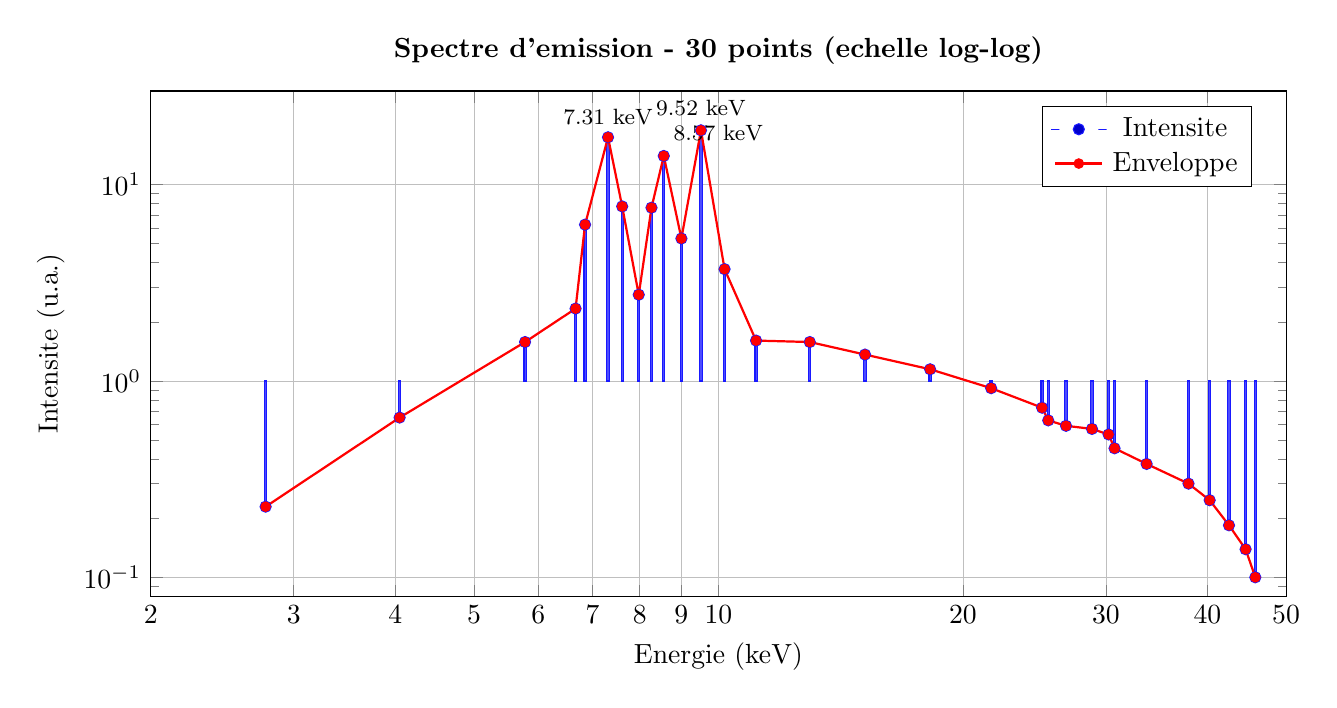
\begin{tikzpicture}
\begin{axis}[
    width=16cm,
    height=8cm,
    xlabel={Energie (keV)},
    ylabel={Intensite (u.a.)},
    title={\textbf{Spectre d'emission - 30 points (echelle log-log)}},
    xmin=2, xmax=50,
    ymin=0.08, ymax=30,
    xmode=log,
    ymode=log,
    grid=major,
    grid style={line width=.1pt, draw=gray!30},
    major grid style={line width=.2pt,draw=gray!50},
    legend pos=north east,
    xtick={2,3,4,5,6,7,8,9,10,20,30,40,50},
    xticklabels={2,3,4,5,6,7,8,9,10,20,30,40,50},
]

% Barres du spectre
\addplot+[
    ybar,
    bar width=0.8pt,
    fill=blue!70,
    draw=blue!90,
] coordinates {
    (2.770, 0.229)
    (4.050, 0.651)
    (5.780, 1.579)
    (6.670, 2.337)
    (6.852, 6.256)
    (7.313, 17.424)
    (7.613, 7.745)
    (7.979, 2.750)
    (8.272, 7.631)
    (8.565, 14.001)
    (9.004, 5.316)
    (9.517, 18.905)
    (10.176, 3.712)
    (11.127, 1.606)
    (12.957, 1.579)
    (15.154, 1.363)
    (18.228, 1.147)
    (21.669, 0.919)
    (25.037, 0.731)
    (25.476, 0.630)
    (26.793, 0.591)
    (28.843, 0.570)
    (30.234, 0.534)
    (30.747, 0.454)
    (33.675, 0.378)
    (37.921, 0.300)
    (40.263, 0.247)
    (42.533, 0.184)
    (44.583, 0.139)
    (45.827, 0.100)
};
\addlegendentry{Intensite}

% Ligne reliant les points
\addplot[
    color=red,
    mark=*,
    mark size=1.5pt,
    line width=0.8pt,
] coordinates {
    (2.770, 0.229)
    (4.050, 0.651)
    (5.780, 1.579)
    (6.670, 2.337)
    (6.852, 6.256)
    (7.313, 17.424)
    (7.613, 7.745)
    (7.979, 2.750)
    (8.272, 7.631)
    (8.565, 14.001)
    (9.004, 5.316)
    (9.517, 18.905)
    (10.176, 3.712)
    (11.127, 1.606)
    (12.957, 1.579)
    (15.154, 1.363)
    (18.228, 1.147)
    (21.669, 0.919)
    (25.037, 0.731)
    (25.476, 0.630)
    (26.793, 0.591)
    (28.843, 0.570)
    (30.234, 0.534)
    (30.747, 0.454)
    (33.675, 0.378)
    (37.921, 0.300)
    (40.263, 0.247)
    (42.533, 0.184)
    (44.583, 0.139)
    (45.827, 0.100)
};
\addlegendentry{Enveloppe}

% Annotations des pics principaux
\node[above, font=\footnotesize] at (axis cs:9.517,20) {9.52 keV};
\node[above, font=\footnotesize] at (axis cs:7.313,18) {7.31 keV};
\node[above right, font=\footnotesize] at (axis cs:8.565,15) {8.57 keV};
\end{axis}
\end{tikzpicture}
\captionsetup{labelformat=empty}
\caption{\footnotesize Spectre d'emission avec 30 raies entre 2.77 et 45.83 keV (echelle log-log). Les pics principaux sont a 9.52 keV (18.9), 7.31 keV (17.4) et 8.57 keV (14.0). L'echelle logarithmique sur les deux axes permet de visualiser toute la dynamique du spectre.}
\end{figure}

\normalsize
\noindent \begin{mdframed}[backgroundcolor=orange!20]
\subsection{\color{blue}\textbf{Taux d'absorption en fonction de l'energie}\color{black}}
\end{mdframed}
\footnotesize
\medskip

\begin{figure}[H]
\centering
\begin{tikzpicture}[xscale=0.25, yscale=0.06]
% Axes
\draw[->] (0,0) -- (52,0) node[right] {\footnotesize \textbf{Energie (keV)}};
\draw[->] (0,0) -- (0,110) node[above] {\footnotesize \textbf{Probabilite (\%)}};
% Graduations X
\foreach \x in {10,20,30,40,50} \draw (\x,0) -- (\x,-2) node[below] {\x};
% Graduations Y
\foreach \y in {20,40,60,80,100} \draw (0,\y) -- (-1,\y) node[left] {\y};
% Lignes de reference
\draw[dashed, gray] (0,50) -- (50,50);
\draw[dashed, orange] (0,10) -- (50,10);
% Courbe absorption (rouge)
\draw[red, thick] (3,100) -- (10,100) -- (13,92) -- (15,80) -- (18,64) -- (22,50) -- (25,41) -- (29,33) -- (34,28) -- (40,23) -- (46,21);
% Courbe transmission (bleu)
\draw[blue, thick] (3,0) -- (10,1) -- (13,8) -- (15,20) -- (18,36) -- (22,50) -- (25,59) -- (29,67) -- (34,72) -- (40,77) -- (46,78);
% Legende
\draw[red, thick] (35,95) -- (38,95) node[right, black] {\small \textbf{Absorption}};
\draw[blue, thick] (35,88) -- (38,88) node[right, black] {\small \textbf{Transmission}};
\end{tikzpicture}
\captionsetup{labelformat=empty}
\caption{\footnotesize Absorption et transmission dans 1 cm d'eau.}
\end{figure}

\begin{table}[H]
\centering
\caption{Probabilite d'absorption dans 1 cm d'eau -- Spectre 30 points}
\label{tab:absorption_30pts}
\footnotesize
\begin{tabular}{@{}c c c c c c | c c c c c c@{}}
\toprule
\textbf{N°} & \textbf{E (keV)} & \textbf{I} & $\bm{\mu}$ & \textbf{P(\%)} & \textbf{T(\%)} &
\textbf{N°} & \textbf{E (keV)} & \textbf{I} & $\bm{\mu}$ & \textbf{P(\%)} & \textbf{T(\%)} \\
\midrule
\cellcolor{red!15}{\footnotesize 1} & \cellcolor{red!15}{\footnotesize 2.77} & \cellcolor{red!15}{\footnotesize 0.23} & \cellcolor{red!15}{\footnotesize 242.7} & \cellcolor{red!15}{\footnotesize $\sim$100} & \cellcolor{red!15}{\footnotesize $\sim$0} &
\cellcolor{orange!15}{\footnotesize 16} & \cellcolor{orange!15}{\footnotesize 15.15} & \cellcolor{orange!15}{\footnotesize 1.36} & \cellcolor{orange!15}{\footnotesize 1.63} & \cellcolor{orange!15}{\footnotesize 80.4} & \cellcolor{orange!15}{\footnotesize 19.6} \\
\cellcolor{red!15}{\footnotesize 2} & \cellcolor{red!15}{\footnotesize 4.05} & \cellcolor{red!15}{\footnotesize 0.65} & \cellcolor{red!15}{\footnotesize 79.7} & \cellcolor{red!15}{\footnotesize $\sim$100} & \cellcolor{red!15}{\footnotesize $\sim$0} &
\cellcolor{yellow!15}{\footnotesize 17} & \cellcolor{yellow!15}{\footnotesize 18.23} & \cellcolor{yellow!15}{\footnotesize 1.15} & \cellcolor{yellow!15}{\footnotesize 1.02} & \cellcolor{yellow!15}{\footnotesize 64.0} & \cellcolor{yellow!15}{\footnotesize 36.0} \\
\cellcolor{red!15}{\footnotesize 3} & \cellcolor{red!15}{\footnotesize 5.78} & \cellcolor{red!15}{\footnotesize 1.58} & \cellcolor{red!15}{\footnotesize 26.7} & \cellcolor{red!15}{\footnotesize $\sim$100} & \cellcolor{red!15}{\footnotesize $\sim$0} &
\cellcolor{yellow!15}{\footnotesize 18} & \cellcolor{yellow!15}{\footnotesize 21.67} & \cellcolor{yellow!15}{\footnotesize 0.92} & \cellcolor{yellow!15}{\footnotesize 0.70} & \cellcolor{yellow!15}{\footnotesize 50.1} & \cellcolor{yellow!15}{\footnotesize 49.9} \\
\cellcolor{red!15}{\footnotesize 4} & \cellcolor{red!15}{\footnotesize 6.67} & \cellcolor{red!15}{\footnotesize 2.34} & \cellcolor{red!15}{\footnotesize 17.2} & \cellcolor{red!15}{\footnotesize $\sim$100} & \cellcolor{red!15}{\footnotesize $\sim$0} &
\cellcolor{yellow!15}{\footnotesize 19} & \cellcolor{yellow!15}{\footnotesize 25.04} & \cellcolor{yellow!15}{\footnotesize 0.73} & \cellcolor{yellow!15}{\footnotesize 0.53} & \cellcolor{yellow!15}{\footnotesize 41.1} & \cellcolor{yellow!15}{\footnotesize 58.9} \\
\cellcolor{red!15}{\footnotesize 5} & \cellcolor{red!15}{\footnotesize 6.85} & \cellcolor{red!15}{\footnotesize 6.26} & \cellcolor{red!15}{\footnotesize 15.9} & \cellcolor{red!15}{\footnotesize $\sim$100} & \cellcolor{red!15}{\footnotesize $\sim$0} &
\cellcolor{yellow!15}{\footnotesize 20} & \cellcolor{yellow!15}{\footnotesize 25.48} & \cellcolor{yellow!15}{\footnotesize 0.63} & \cellcolor{yellow!15}{\footnotesize 0.51} & \cellcolor{yellow!15}{\footnotesize 40.1} & \cellcolor{yellow!15}{\footnotesize 59.9} \\
\cellcolor{red!15}{\footnotesize 6} & \cellcolor{red!15}{\footnotesize 7.31} & \cellcolor{red!15}{\footnotesize \textbf{17.42}} & \cellcolor{red!15}{\footnotesize 13.0} & \cellcolor{red!15}{\footnotesize $\sim$100} & \cellcolor{red!15}{\footnotesize $\sim$0} &
\cellcolor{yellow!15}{\footnotesize 21} & \cellcolor{yellow!15}{\footnotesize 26.79} & \cellcolor{yellow!15}{\footnotesize 0.59} & \cellcolor{yellow!15}{\footnotesize 0.47} & \cellcolor{yellow!15}{\footnotesize 37.2} & \cellcolor{yellow!15}{\footnotesize 62.8} \\
\cellcolor{red!15}{\footnotesize 7} & \cellcolor{red!15}{\footnotesize 7.61} & \cellcolor{red!15}{\footnotesize 7.75} & \cellcolor{red!15}{\footnotesize 11.5} & \cellcolor{red!15}{\footnotesize $\sim$100} & \cellcolor{red!15}{\footnotesize $\sim$0} &
\cellcolor{yellow!15}{\footnotesize 22} & \cellcolor{yellow!15}{\footnotesize 28.84} & \cellcolor{yellow!15}{\footnotesize 0.57} & \cellcolor{yellow!15}{\footnotesize 0.40} & \cellcolor{yellow!15}{\footnotesize 33.3} & \cellcolor{yellow!15}{\footnotesize 66.7} \\
\cellcolor{red!15}{\footnotesize 8} & \cellcolor{red!15}{\footnotesize 7.98} & \cellcolor{red!15}{\footnotesize 2.75} & \cellcolor{red!15}{\footnotesize 10.0} & \cellcolor{red!15}{\footnotesize $\sim$100} & \cellcolor{red!15}{\footnotesize $\sim$0} &
\cellcolor{green!15}{\footnotesize 23} & \cellcolor{green!15}{\footnotesize 30.23} & \cellcolor{green!15}{\footnotesize 0.53} & \cellcolor{green!15}{\footnotesize 0.37} & \cellcolor{green!15}{\footnotesize 31.1} & \cellcolor{green!15}{\footnotesize 68.9} \\
\cellcolor{red!15}{\footnotesize 9} & \cellcolor{red!15}{\footnotesize 8.27} & \cellcolor{red!15}{\footnotesize 7.63} & \cellcolor{red!15}{\footnotesize 9.04} & \cellcolor{red!15}{\footnotesize 100.0} & \cellcolor{red!15}{\footnotesize 0.0} &
\cellcolor{green!15}{\footnotesize 24} & \cellcolor{green!15}{\footnotesize 30.75} & \cellcolor{green!15}{\footnotesize 0.45} & \cellcolor{green!15}{\footnotesize 0.37} & \cellcolor{green!15}{\footnotesize 30.6} & \cellcolor{green!15}{\footnotesize 69.4} \\
\cellcolor{red!15}{\footnotesize 10} & \cellcolor{red!15}{\footnotesize 8.57} & \cellcolor{red!15}{\footnotesize \textbf{14.00}} & \cellcolor{red!15}{\footnotesize 8.20} & \cellcolor{red!15}{\footnotesize 100.0} & \cellcolor{red!15}{\footnotesize 0.0} &
\cellcolor{green!15}{\footnotesize 25} & \cellcolor{green!15}{\footnotesize 33.68} & \cellcolor{green!15}{\footnotesize 0.38} & \cellcolor{green!15}{\footnotesize 0.33} & \cellcolor{green!15}{\footnotesize 28.0} & \cellcolor{green!15}{\footnotesize 72.0} \\
\cellcolor{red!15}{\footnotesize 11} & \cellcolor{red!15}{\footnotesize 9.00} & \cellcolor{red!15}{\footnotesize 5.32} & \cellcolor{red!15}{\footnotesize 7.14} & \cellcolor{red!15}{\footnotesize 99.9} & \cellcolor{red!15}{\footnotesize 0.1} &
\cellcolor{green!15}{\footnotesize 26} & \cellcolor{green!15}{\footnotesize 37.92} & \cellcolor{green!15}{\footnotesize 0.30} & \cellcolor{green!15}{\footnotesize 0.29} & \cellcolor{green!15}{\footnotesize 24.8} & \cellcolor{green!15}{\footnotesize 75.2} \\
\cellcolor{red!15}{\footnotesize 12} & \cellcolor{red!15}{\footnotesize 9.52} & \cellcolor{red!15}{\footnotesize \textbf{18.91}} & \cellcolor{red!15}{\footnotesize 6.12} & \cellcolor{red!15}{\footnotesize 99.8} & \cellcolor{red!15}{\footnotesize 0.2} &
\cellcolor{green!15}{\footnotesize 27} & \cellcolor{green!15}{\footnotesize 40.26} & \cellcolor{green!15}{\footnotesize 0.25} & \cellcolor{green!15}{\footnotesize 0.27} & \cellcolor{green!15}{\footnotesize 23.4} & \cellcolor{green!15}{\footnotesize 76.6} \\
\cellcolor{orange!15}{\footnotesize 13} & \cellcolor{orange!15}{\footnotesize 10.18} & \cellcolor{orange!15}{\footnotesize 3.71} & \cellcolor{orange!15}{\footnotesize 5.07} & \cellcolor{orange!15}{\footnotesize 99.4} & \cellcolor{orange!15}{\footnotesize 0.6} &
\cellcolor{green!15}{\footnotesize 28} & \cellcolor{green!15}{\footnotesize 42.53} & \cellcolor{green!15}{\footnotesize 0.18} & \cellcolor{green!15}{\footnotesize 0.26} & \cellcolor{green!15}{\footnotesize 22.6} & \cellcolor{green!15}{\footnotesize 77.4} \\
\cellcolor{orange!15}{\footnotesize 14} & \cellcolor{orange!15}{\footnotesize 11.13} & \cellcolor{orange!15}{\footnotesize 1.61} & \cellcolor{orange!15}{\footnotesize 3.93} & \cellcolor{orange!15}{\footnotesize 98.0} & \cellcolor{orange!15}{\footnotesize 2.0} &
\cellcolor{green!15}{\footnotesize 29} & \cellcolor{green!15}{\footnotesize 44.58} & \cellcolor{green!15}{\footnotesize 0.14} & \cellcolor{green!15}{\footnotesize 0.25} & \cellcolor{green!15}{\footnotesize 21.9} & \cellcolor{green!15}{\footnotesize 78.1} \\
\cellcolor{orange!15}{\footnotesize 15} & \cellcolor{orange!15}{\footnotesize 12.96} & \cellcolor{orange!15}{\footnotesize 1.58} & \cellcolor{orange!15}{\footnotesize 2.54} & \cellcolor{orange!15}{\footnotesize 92.1} & \cellcolor{orange!15}{\footnotesize 7.9} &
\cellcolor{green!15}{\footnotesize 30} & \cellcolor{green!15}{\footnotesize 45.83} & \cellcolor{green!15}{\footnotesize 0.10} & \cellcolor{green!15}{\footnotesize 0.24} & \cellcolor{green!15}{\footnotesize 21.5} & \cellcolor{green!15}{\footnotesize 78.5} \\
\bottomrule
\end{tabular}
\end{table}

\vspace{0.2cm}
\footnotesize
\noindent \color{blue}\textbf{Legende :}\color{black} E = Energie, I = Intensite (u.a.), $\mu$ = coefficient d'attenuation (cm$^{-1}$), P = Absorption (\%), T = Transmission (\%)
\noindent \color{blue}\textbf{Code couleur :}\color{black} 
\noindent \colorbox{red!15}{$>$99\%} 
\noindent \colorbox{orange!15}{90--99\%} 
\noindent \colorbox{yellow!15}{30--90\%} 
\noindent \colorbox{green!15}{$<$30\%}

\normalsize
\noindent \begin{mdframed}[backgroundcolor=orange!20]
\subsection{\color{blue}\textbf{Resultats}\color{black}}
\end{mdframed}
\footnotesize
\medskip

\begin{table}[H]
\centering
\captionsetup{labelformat=empty}
\caption{\footnotesize Moyenne ponderee par l'intensite}
\begin{tabular}{@{}l c@{}}
\toprule
\footnotesize \textbf{Grandeur} &\footnotesize \textbf{Valeur} \\
\midrule
\footnotesize Intensite totale &\footnotesize 100.0 (u.a.) \\
\footnotesize \textbf{Absorption moyenne (1 cm eau)} &\footnotesize \textbf{95.37\%} \\
\footnotesize Transmission moyenne &\footnotesize  4.63\% \\
\bottomrule
\end{tabular}
\end{table}

\begin{table}[H]
\centering
\captionsetup{labelformat=empty}
\caption{\footnotesize Analyse par gamme d'energie}
\begin{tabular}{@{}l c c c@{}}
\toprule
\footnotesize \textbf{Gamme} &\footnotesize \textbf{Intensite} &\footnotesize \textbf{\% du spectre} &\footnotesize \textbf{P(1 cm)} \\
\midrule
\rowcolor{red!15}
\footnotesize 0--10 keV &\footnotesize 84.8 &\footnotesize 84.8\% &\footnotesize 99.94\% \\
\rowcolor{orange!15}
\footnotesize 10--20 keV &\footnotesize 9.4 &\footnotesize 9.4\% &\footnotesize 90.87\% \\
\rowcolor{yellow!15}
\footnotesize 20--30 keV &\footnotesize 3.4 &\footnotesize 3.4\% &\footnotesize 41.35\% \\
\rowcolor{green!15}
\footnotesize 30--50 keV &\footnotesize 2.3 &\footnotesize 2.3\% &\footnotesize 27.25\% \\
\bottomrule
\end{tabular}
\end{table}

\normalsize
\noindent \begin{mdframed}[backgroundcolor=orange!20]
\subsection{\color{blue}\textbf{Conclusions}\color{black}}
\end{mdframed}
\footnotesize
\medskip

\begin{tcolorbox}[colback=blue!5,colframe=blue!75!black,title=\textbf{Synthese}]

\noindent \color{blue}\textbf{Caracteristiques du spectre :}\color{black}

\begin{itemize}
\item Spectre domine par des rayons X de basse energie (7--10 keV)
\item Pics principaux : 9.52 keV (18.9\%), 7.31 keV (17.4\%), 8.57 keV (14.0\%)
\item 84.8\% de l'intensite est concentree en dessous de 10 keV
\end{itemize}

\vspace{0.1cm}

\noindent \color{blue}\textbf{Absorption dans 1 cm d'eau :}\color{black}
\begin{itemize}
\item Les photons $< 10$ keV sont \textbf{totalement absorbes} ($>$99.9\%)
\item L'absorption chute rapidement entre 10 et 25 keV (de 99\% a 40\%)
\item Les photons $> 30$ keV ont une absorption moderee ($\sim$25--30\%)
\item \textbf{Absorption moyenne ponderee : 95.4\%}
\end{itemize}

\vspace{0.1cm}

\noindent \color{blue}\textbf{Consequence pratique :}\color{black}
\noindent Avec ce spectre, \color{blue}\textbf{1 cm d'eau suffit} pour absorber 95\% des photons emis, grace a la predominance des rayons X de basse energie.

\end{tcolorbox}


\clearpage

%==============================================================================
\normalsize
\noindent \begin{mdframed}[backgroundcolor=orange!20]
\section{\Large \color{blue} \textbf{Probabilite d'absorption dans 5 mm d'eau \\ Spectre MiniX 30 points}\color{black}}
\end{mdframed}
\footnotesize
%==============================================================================

\begin{figure}[H]
\centering
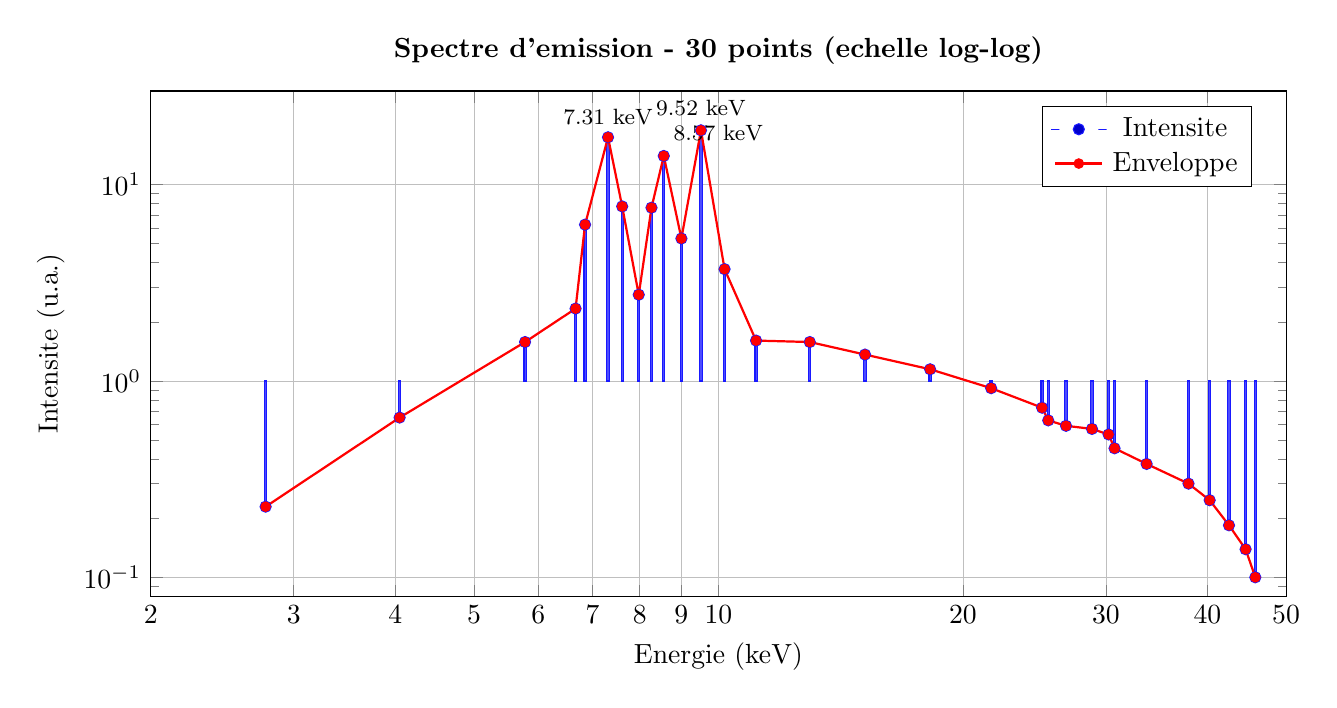
\begin{tikzpicture}
\begin{axis}[
    width=16cm,
    height=8cm,
    xlabel={Energie (keV)},
    ylabel={Intensite (u.a.)},
    title={\textbf{Spectre d'emission - 30 points (echelle log-log)}},
    xmin=2, xmax=50,
    ymin=0.08, ymax=30,
    xmode=log,
    ymode=log,
    grid=major,
    grid style={line width=.1pt, draw=gray!30},
    major grid style={line width=.2pt,draw=gray!50},
    legend pos=north east,
    xtick={2,3,4,5,6,7,8,9,10,20,30,40,50},
    xticklabels={2,3,4,5,6,7,8,9,10,20,30,40,50},
]

% Barres du spectre
\addplot+[
    ybar,
    bar width=0.8pt,
    fill=blue!70,
    draw=blue!90,
] coordinates {
    (2.770, 0.229)
    (4.050, 0.651)
    (5.780, 1.579)
    (6.670, 2.337)
    (6.852, 6.256)
    (7.313, 17.424)
    (7.613, 7.745)
    (7.979, 2.750)
    (8.272, 7.631)
    (8.565, 14.001)
    (9.004, 5.316)
    (9.517, 18.905)
    (10.176, 3.712)
    (11.127, 1.606)
    (12.957, 1.579)
    (15.154, 1.363)
    (18.228, 1.147)
    (21.669, 0.919)
    (25.037, 0.731)
    (25.476, 0.630)
    (26.793, 0.591)
    (28.843, 0.570)
    (30.234, 0.534)
    (30.747, 0.454)
    (33.675, 0.378)
    (37.921, 0.300)
    (40.263, 0.247)
    (42.533, 0.184)
    (44.583, 0.139)
    (45.827, 0.100)
};
\addlegendentry{Intensite}

% Ligne reliant les points
\addplot[
    color=red,
    mark=*,
    mark size=1.5pt,
    line width=0.8pt,
] coordinates {
    (2.770, 0.229)
    (4.050, 0.651)
    (5.780, 1.579)
    (6.670, 2.337)
    (6.852, 6.256)
    (7.313, 17.424)
    (7.613, 7.745)
    (7.979, 2.750)
    (8.272, 7.631)
    (8.565, 14.001)
    (9.004, 5.316)
    (9.517, 18.905)
    (10.176, 3.712)
    (11.127, 1.606)
    (12.957, 1.579)
    (15.154, 1.363)
    (18.228, 1.147)
    (21.669, 0.919)
    (25.037, 0.731)
    (25.476, 0.630)
    (26.793, 0.591)
    (28.843, 0.570)
    (30.234, 0.534)
    (30.747, 0.454)
    (33.675, 0.378)
    (37.921, 0.300)
    (40.263, 0.247)
    (42.533, 0.184)
    (44.583, 0.139)
    (45.827, 0.100)
};
\addlegendentry{Enveloppe}

% Annotations des pics principaux
\node[above, font=\footnotesize] at (axis cs:9.517,20) {9.52 keV};
\node[above, font=\footnotesize] at (axis cs:7.313,18) {7.31 keV};
\node[above right, font=\footnotesize] at (axis cs:8.565,15) {8.57 keV};

\end{axis}
\end{tikzpicture}
\captionsetup{labelformat=empty}
\caption{Spectre d'emission avec 30 raies entre 2.77 et 45.83 keV (echelle log-log). Les pics principaux sont a 9.52 keV (18.9), 7.31 keV (17.4) et 8.57 keV (14.0).}
\end{figure}


\normalsize
\noindent \begin{mdframed}[backgroundcolor=orange!20]
\subsection{\color{blue}\textbf{Taux d'absorption en fonction de l'energie}\color{black}}
\end{mdframed}
\footnotesize
\medskip


\begin{figure}[H]
\centering
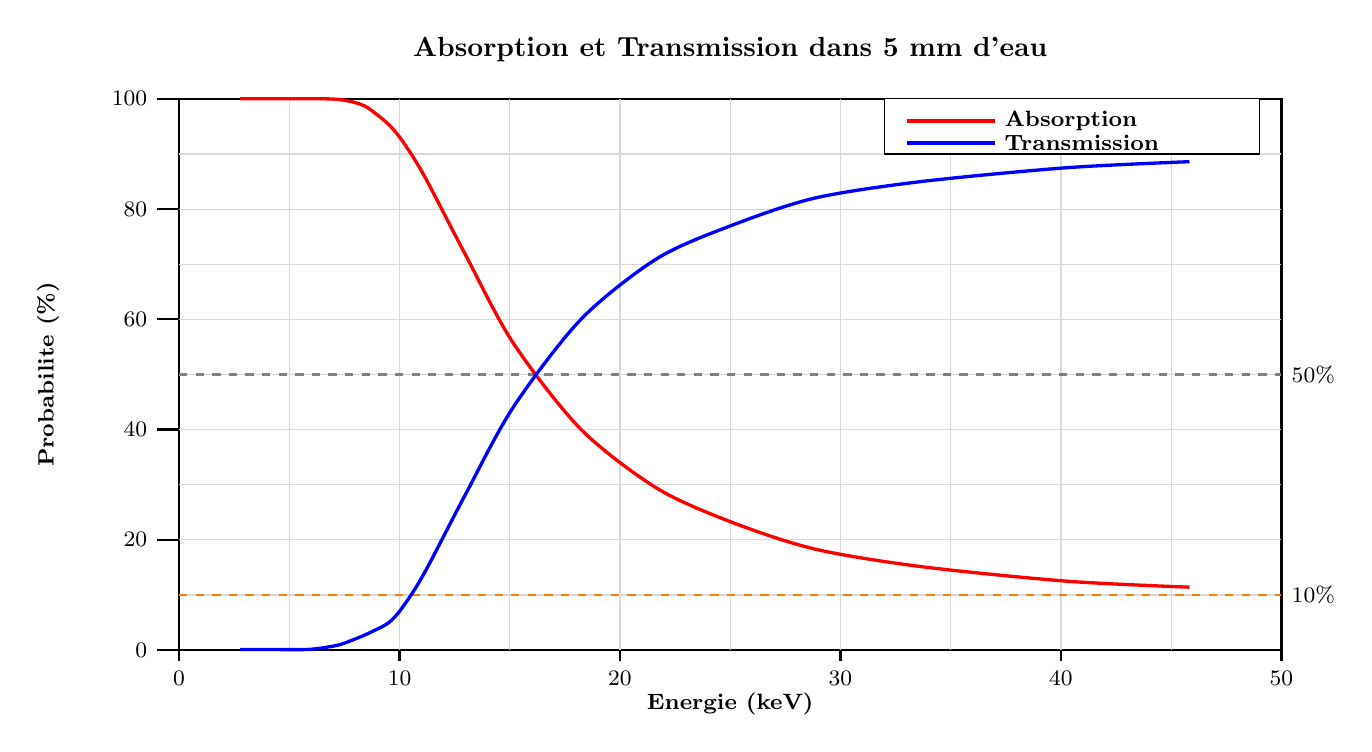
\begin{tikzpicture}[x=0.28cm, y=0.07cm]
% Cadre
\draw[thick] (0,0) rectangle (50,100);

% Grille horizontale
\foreach \y in {10,20,30,40,50,60,70,80,90} {
    \draw[gray!30, thin] (0,\y) -- (50,\y);
}
% Grille verticale
\foreach \x in {5,10,15,20,25,30,35,40,45} {
    \draw[gray!30, thin] (\x,0) -- (\x,100);
}

% Lignes de reference
\draw[dashed, gray, thick] (0,50) -- (50,50) node[right, black, font=\footnotesize] {50\%};
\draw[dashed, orange, thick] (0,10) -- (50,10) node[right, black, font=\footnotesize] {10\%};

% Axe X - graduations
\foreach \x/\label in {0/0, 10/10, 20/20, 30/30, 40/40, 50/50} {
    \draw[thick] (\x,0) -- (\x,-2);
    \node[below, font=\footnotesize] at (\x,-2) {\label};
}
% Axe Y - graduations
\foreach \y/\label in {0/0, 20/20, 40/40, 60/60, 80/80, 100/100} {
    \draw[thick] (0,\y) -- (-1,\y);
    \node[left, font=\footnotesize] at (-1,\y) {\label};
}

% Labels des axes
\node[below, font=\small] at (25,-6) {\footnotesize \textbf{Energie (keV)}};
\node[rotate=90, above, font=\small] at (-5,50) {\footnotesize \textbf{Probabilite (\%)}};

% Titre
\node[above, font=\bfseries] at (25,105) {Absorption et Transmission dans 5 mm d'eau};

% Courbe d'absorption (rouge)
\draw[red, very thick] 
    plot[smooth, tension=0.5] coordinates {
        (2.77, 100) (4.05, 100) (5.78, 100) (6.67, 100) (7.31, 99.85)
        (7.98, 99.33) (8.57, 98.35) (9.52, 95.30) (10.18, 92.07)
        (11.13, 85.97) (12.96, 71.95) (15.15, 55.75) (18.23, 40.04)
        (21.67, 29.37) (25.04, 23.24) (28.84, 18.32) (33.68, 15.13)
        (40.26, 12.50) (45.83, 11.41)
    };

% Courbe de transmission (bleu)
\draw[blue, very thick] 
    plot[smooth, tension=0.5] coordinates {
        (2.77, 0.1) (4.05, 0.1) (5.78, 0.1) (6.67, 0.5) (7.31, 1)
        (7.98, 2) (8.57, 3) (9.52, 5) (10.18, 8)
        (11.13, 14) (12.96, 28) (15.15, 44) (18.23, 60)
        (21.67, 71) (25.04, 77) (28.84, 82) (33.68, 85)
        (40.26, 87.5) (45.83, 88.6)
    };

% Legende
\fill[white] (32,90) rectangle (49,100);
\draw (32,90) rectangle (49,100);
\draw[red, very thick] (33,96) -- (37,96);
\node[right, font=\footnotesize] at (37,96) {\footnotesize \textbf{Absorption}};
\draw[blue, very thick] (33,92) -- (37,92);
\node[right, font=\footnotesize] at (37,92) {\footnotesize \textbf{Transmission}};

\end{tikzpicture}
\caption{\footnotesize Probabilite d'absorption (rouge) et de transmission (bleu) dans 5 mm d'eau. Les photons $< 8$ keV sont quasi-totalement absorbes. La transmission atteint 50\% vers 16 keV.}
\end{figure}

%\begin{comment}

\begin{table}[H]
\centering
\captionsetup{labelformat=empty}
\caption{\footnotesize Probabilite d'absorption dans 5 mm d'eau -- Spectre 30 points}
\footnotesize
\begin{tabular}{@{}c c c c c c | c c c c c c@{}}
\toprule
\footnotesize\textbf{N} & \footnotesize\textbf{E (keV)} & \footnotesize\textbf{I} & \footnotesize$\bm{\mu}$ & \footnotesize\textbf{P(\%)} & \footnotesize\textbf{T(\%)} &
\footnotesize\textbf{N} & \footnotesize\textbf{E (keV)} & \footnotesize\textbf{I} & \footnotesize$\bm{\mu}$ & \footnotesize\textbf{P(\%)} & \footnotesize\textbf{T(\%)} \\
\midrule
\cellcolor{red!15}{\footnotesize 1} & \cellcolor{red!15}{\footnotesize 2.77} & \cellcolor{red!15}{\footnotesize 0.23} & \cellcolor{red!15}{\footnotesize 242.7} & \cellcolor{red!15}{\footnotesize $\sim$100} & \cellcolor{red!15}{\footnotesize $\sim$0} &
\cellcolor{orange!15}{\footnotesize 16} & \cellcolor{orange!15}{\footnotesize 15.15} & \cellcolor{orange!15}{\footnotesize 1.36} & \cellcolor{orange!15}{\footnotesize 1.63} & \cellcolor{orange!15}{\footnotesize 55.8} & \cellcolor{orange!15}{\footnotesize 44.2} \\
\cellcolor{red!15}{\footnotesize 2} & \cellcolor{red!15}{\footnotesize 4.05} & \cellcolor{red!15}{\footnotesize 0.65} & \cellcolor{red!15}{\footnotesize 79.7} & \cellcolor{red!15}{\footnotesize $\sim$100} & \cellcolor{red!15}{\footnotesize $\sim$0} &
\cellcolor{yellow!15}{\footnotesize 17} & \cellcolor{yellow!15}{\footnotesize 18.23} & \cellcolor{yellow!15}{\footnotesize 1.15} & \cellcolor{yellow!15}{\footnotesize 1.02} & \cellcolor{yellow!15}{\footnotesize 40.0} & \cellcolor{yellow!15}{\footnotesize 60.0} \\
\cellcolor{red!15}{\footnotesize 3} & \cellcolor{red!15}{\footnotesize 5.78} & \cellcolor{red!15}{\footnotesize 1.58} & \cellcolor{red!15}{\footnotesize 26.7} & \cellcolor{red!15}{\footnotesize $\sim$100} & \cellcolor{red!15}{\footnotesize $\sim$0} &
\cellcolor{yellow!15}{\footnotesize 18} & \cellcolor{yellow!15}{\footnotesize 21.67} & \cellcolor{yellow!15}{\footnotesize 0.92} & \cellcolor{yellow!15}{\footnotesize 0.70} & \cellcolor{yellow!15}{\footnotesize 29.4} & \cellcolor{yellow!15}{\footnotesize 70.6} \\
\cellcolor{red!15}{\footnotesize 4} & \cellcolor{red!15}{\footnotesize 6.67} & \cellcolor{red!15}{\footnotesize 2.34} & \cellcolor{red!15}{\footnotesize 17.2} & \cellcolor{red!15}{\footnotesize 100.0} & \cellcolor{red!15}{\footnotesize 0.0} &
\cellcolor{yellow!15}{\footnotesize 19} & \cellcolor{yellow!15}{\footnotesize 25.04} & \cellcolor{yellow!15}{\footnotesize 0.73} & \cellcolor{yellow!15}{\footnotesize 0.53} & \cellcolor{yellow!15}{\footnotesize 23.2} & \cellcolor{yellow!15}{\footnotesize 76.8} \\
\cellcolor{red!15}{\footnotesize 5} & \cellcolor{red!15}{\footnotesize 6.85} & \cellcolor{red!15}{\footnotesize 6.26} & \cellcolor{red!15}{\footnotesize 15.9} & \cellcolor{red!15}{\footnotesize 100.0} & \cellcolor{red!15}{\footnotesize 0.0} &
\cellcolor{yellow!15}{\footnotesize 20} & \cellcolor{yellow!15}{\footnotesize 25.48} & \cellcolor{yellow!15}{\footnotesize 0.63} & \cellcolor{yellow!15}{\footnotesize 0.51} & \cellcolor{yellow!15}{\footnotesize 22.6} & \cellcolor{yellow!15}{\footnotesize 77.4} \\
\cellcolor{red!15}{\footnotesize 6} & \cellcolor{red!15}{\footnotesize 7.31} & \cellcolor{red!15}{\footnotesize \textbf{17.42}} & \cellcolor{red!15}{\footnotesize 13.0} & \cellcolor{red!15}{\footnotesize 99.9} & \cellcolor{red!15}{\footnotesize 0.1} &
\cellcolor{yellow!15}{\footnotesize 21} & \cellcolor{yellow!15}{\footnotesize 26.79} & \cellcolor{yellow!15}{\footnotesize 0.59} & \cellcolor{yellow!15}{\footnotesize 0.47} & \cellcolor{yellow!15}{\footnotesize 20.8} & \cellcolor{yellow!15}{\footnotesize 79.2} \\
\cellcolor{red!15}{\footnotesize 7} & \cellcolor{red!15}{\footnotesize 7.61} & \cellcolor{red!15}{\footnotesize 7.75} & \cellcolor{red!15}{\footnotesize 11.5} & \cellcolor{red!15}{\footnotesize 99.7} & \cellcolor{red!15}{\footnotesize 0.3} &
\cellcolor{green!15}{\footnotesize 22} & \cellcolor{green!15}{\footnotesize 28.84} & \cellcolor{green!15}{\footnotesize 0.57} & \cellcolor{green!15}{\footnotesize 0.40} & \cellcolor{green!15}{\footnotesize 18.3} & \cellcolor{green!15}{\footnotesize 81.7} \\
\cellcolor{red!15}{\footnotesize 8} & \cellcolor{red!15}{\footnotesize 7.98} & \cellcolor{red!15}{\footnotesize 2.75} & \cellcolor{red!15}{\footnotesize 10.0} & \cellcolor{red!15}{\footnotesize 99.3} & \cellcolor{red!15}{\footnotesize 0.7} &
\cellcolor{green!15}{\footnotesize 23} & \cellcolor{green!15}{\footnotesize 30.23} & \cellcolor{green!15}{\footnotesize 0.53} & \cellcolor{green!15}{\footnotesize 0.37} & \cellcolor{green!15}{\footnotesize 17.0} & \cellcolor{green!15}{\footnotesize 83.0} \\
\cellcolor{red!15}{\footnotesize 9} & \cellcolor{red!15}{\footnotesize 8.27} & \cellcolor{red!15}{\footnotesize 7.63} & \cellcolor{red!15}{\footnotesize 9.04} & \cellcolor{red!15}{\footnotesize 98.9} & \cellcolor{red!15}{\footnotesize 1.1} &
\cellcolor{green!15}{\footnotesize 24} & \cellcolor{green!15}{\footnotesize 30.75} & \cellcolor{green!15}{\footnotesize 0.45} & \cellcolor{green!15}{\footnotesize 0.37} & \cellcolor{green!15}{\footnotesize 16.7} & \cellcolor{green!15}{\footnotesize 83.3} \\
\cellcolor{red!15}{\footnotesize 10} & \cellcolor{red!15}{\footnotesize 8.57} & \cellcolor{red!15}{\footnotesize \textbf{14.00}} & \cellcolor{red!15}{\footnotesize 8.20} & \cellcolor{red!15}{\footnotesize 98.4} & \cellcolor{red!15}{\footnotesize 1.6} &
\cellcolor{green!15}{\footnotesize 25} & \cellcolor{green!15}{\footnotesize 33.68} & \cellcolor{green!15}{\footnotesize 0.38} & \cellcolor{green!15}{\footnotesize 0.33} & \cellcolor{green!15}{\footnotesize 15.1} & \cellcolor{green!15}{\footnotesize 84.9} \\
\cellcolor{red!15}{\footnotesize 11} & \cellcolor{red!15}{\footnotesize 9.00} & \cellcolor{red!15}{\footnotesize 5.32} & \cellcolor{red!15}{\footnotesize 7.14} & \cellcolor{red!15}{\footnotesize 97.2} & \cellcolor{red!15}{\footnotesize 2.8} &
\cellcolor{green!15}{\footnotesize 26} & \cellcolor{green!15}{\footnotesize 37.92} & \cellcolor{green!15}{\footnotesize 0.30} & \cellcolor{green!15}{\footnotesize 0.29} & \cellcolor{green!15}{\footnotesize 13.3} & \cellcolor{green!15}{\footnotesize 86.7} \\
\cellcolor{orange!15}{\footnotesize 12} & \cellcolor{orange!15}{\footnotesize 9.52} & \cellcolor{orange!15}{\footnotesize \textbf{18.91}} & \cellcolor{orange!15}{\footnotesize 6.12} & \cellcolor{orange!15}{\footnotesize 95.3} & \cellcolor{orange!15}{\footnotesize 4.7} &
\cellcolor{green!15}{\footnotesize 27} & \cellcolor{green!15}{\footnotesize 40.26} & \cellcolor{green!15}{\footnotesize 0.25} & \cellcolor{green!15}{\footnotesize 0.27} & \cellcolor{green!15}{\footnotesize 12.5} & \cellcolor{green!15}{\footnotesize 87.5} \\
\cellcolor{orange!15}{\footnotesize 13} & \cellcolor{orange!15}{\footnotesize 10.18} & \cellcolor{orange!15}{\footnotesize 3.71} & \cellcolor{orange!15}{\footnotesize 5.07} & \cellcolor{orange!15}{\footnotesize 92.1} & \cellcolor{orange!15}{\footnotesize 7.9} &
\cellcolor{green!15}{\footnotesize 28} & \cellcolor{green!15}{\footnotesize 42.53} & \cellcolor{green!15}{\footnotesize 0.18} & \cellcolor{green!15}{\footnotesize 0.26} & \cellcolor{green!15}{\footnotesize 12.0} & \cellcolor{green!15}{\footnotesize 88.0} \\
\cellcolor{orange!15}{\footnotesize 14} & \cellcolor{orange!15}{\footnotesize 11.13} & \cellcolor{orange!15}{\footnotesize 1.61} & \cellcolor{orange!15}{\footnotesize 3.93} & \cellcolor{orange!15}{\footnotesize 86.0} & \cellcolor{orange!15}{\footnotesize 14.0} &
\cellcolor{green!15}{\footnotesize 29} & \cellcolor{green!15}{\footnotesize 44.58} & \cellcolor{green!15}{\footnotesize 0.14} & \cellcolor{green!15}{\footnotesize 0.25} & \cellcolor{green!15}{\footnotesize 11.6} & \cellcolor{green!15}{\footnotesize 88.4} \\
\cellcolor{orange!15}{\footnotesize 15} & \cellcolor{orange!15}{\footnotesize 12.96} & \cellcolor{orange!15}{\footnotesize 1.58} & \cellcolor{orange!15}{\footnotesize 2.54} & \cellcolor{orange!15}{\footnotesize 72.0} & \cellcolor{orange!15}{\footnotesize 28.0} &
\cellcolor{green!15}{\footnotesize 30} & \cellcolor{green!15}{\footnotesize 45.83} & \cellcolor{green!15}{\footnotesize 0.10} & \cellcolor{green!15}{\footnotesize 0.24} & \cellcolor{green!15}{\footnotesize 11.4} & \cellcolor{green!15}{\footnotesize 88.6} \\
\bottomrule
\end{tabular}
\end{table}

\vspace{0.2cm}
\footnotesize
\noindent \textbf{Legende :} E = Energie, I = Intensite (u.a.), $\mu$ = coefficient d'attenuation (cm$^{-1}$), P = Absorption (\%), T = Transmission (\%)\\
\noindent \textbf{Code couleur :} 
\colorbox{red!15}{$>$95\%} \quad
\colorbox{orange!15}{50--95\%} \quad
\colorbox{yellow!15}{20--50\%} \quad
\colorbox{green!15}{$<$20\%}

\normalsize
\noindent \begin{mdframed}[backgroundcolor=orange!20]
\subsection{\color{blue}\textbf{Resultats}\color{black}}
\end{mdframed}
\footnotesize
\medskip

\begin{table}[H]
\centering
\captionsetup{labelformat=empty}
\caption{\footnotesize Moyenne ponderee par l'intensite}
\begin{tabular}{@{}l c@{}}
\toprule
\footnotesize \textbf{Grandeur} &\footnotesize \textbf{Valeur} \\
\midrule
\footnotesize Intensite totale &\footnotesize 100.0 (u.a.) \\
\footnotesize \textbf{Absorption moyenne (5 mm eau)} &\footnotesize \textbf{91.70\%} \\
\footnotesize Transmission moyenne &\footnotesize 8.30\% \\
\bottomrule
\end{tabular}
\end{table}

\begin{table}[H]
\centering
\captionsetup{labelformat=empty}
\caption{\footnotesize Analyse par gamme d'energie}
\begin{tabular}{@{}l c c c@{}}
\toprule
\footnotesize \textbf{Gamme} &\footnotesize \textbf{Intensite} &\footnotesize \textbf{\% du spectre} &\footnotesize \textbf{P(5 mm)} \\
\midrule
\rowcolor{red!15}
\footnotesize0--10 keV &\footnotesize 84.8 &\footnotesize 84.8\% &\footnotesize 98.32\% \\
\rowcolor{orange!15}
\footnotesize10--20 keV &\footnotesize 9.4 &\footnotesize 9.4\% &\footnotesize 76.04\% \\
\rowcolor{yellow!15}
\footnotesize20--30 keV &\footnotesize 3.4 &\footnotesize 3.4\% &\footnotesize 23.52\% \\
\rowcolor{green!15}
\footnotesize30--50 keV &\footnotesize 2.3 &\footnotesize 2.3\% &\footnotesize 14.73\% \\
\bottomrule
\end{tabular}
\end{table}

\normalsize
\noindent \begin{mdframed}[backgroundcolor=orange!20]
\subsection{\color{blue}\textbf{Comparaison 5 mm vs 1 cm}\color{black}}
\end{mdframed}
\footnotesize
\medskip

\begin{table}[H]
\centering
\captionsetup{labelformat=empty}
\caption{\footnotesize Comparaison des absorptions pour differentes epaisseurs d'eau}
\begin{tabular}{@{}l c c c@{}}
\toprule
\footnotesize\textbf{Epaisseur} &\footnotesize \textbf{Absorption moyenne} &\footnotesize \textbf{Transmission} &\footnotesize \textbf{Difference} \\
\midrule
\footnotesize 5 mm &\footnotesize 91.70\% &\footnotesize 8.30\% &\footnotesize -- \\
\footnotesize 1 cm &\footnotesize 95.37\% &\footnotesize 4.63\% &\footnotesize +3.67\% \\
\bottomrule
\end{tabular}
\end{table}

\begin{table}[H]
\centering
\captionsetup{labelformat=empty}
\caption{\footnotesize Comparaison par gamme d'energie : 5 mm vs 1 cm}
\begin{tabular}{@{}l c c c@{}}
\toprule
\footnotesize \textbf{Gamme} &\footnotesize \textbf{P(5 mm)} &\footnotesize \textbf{P(1 cm)} &\footnotesize \textbf{Difference} \\
\midrule
\footnotesize 0--10 keV &\footnotesize 98.32\% &\footnotesize 99.94\% &\footnotesize +1.62\% \\
\footnotesize 10--20 keV &\footnotesize 76.04\% &\footnotesize 90.87\% &\footnotesize +14.83\% \\
\footnotesize 20--30 keV &\footnotesize 23.52\% &\footnotesize 41.35\% &\footnotesize +17.83\% \\
\footnotesize 30--50 keV &\footnotesize 14.73\% &\footnotesize 27.25\% &\footnotesize +12.52\% \\
\bottomrule
\end{tabular}
\end{table}

\normalsize
\noindent \begin{mdframed}[backgroundcolor=orange!20]
\subsection{\color{blue}\textbf{Conclusions}\color{black}}
\end{mdframed}
\footnotesize
\medskip

\begin{tcolorbox}[colback=blue!5,colframe=blue!75!black,title=\textbf{Synthese}]
\footnotesize
\noindent \color{blue}\textbf{Caracteristiques du spectre :}\color{black}
\begin{itemize}
\item Spectre domine par des rayons X de basse energie (7--10 keV)
\item 84.8\% de l'intensite est concentree en dessous de 10 keV
\end{itemize}

\vspace{0.1cm}

\noindent \color{blue}\textbf{Absorption dans 5 mm d'eau :}\color{black}
\begin{itemize}
\item Les photons $< 8$ keV sont \textbf{quasi-totalement absorbes} ($>$99\%)
\item L'absorption chute rapidement entre 10 et 20 keV (de 92\% a 40\%)
\item Les photons $> 30$ keV ont une faible absorption ($\sim$11--17\%)
\item \textbf{Absorption moyenne ponderee : 91.7\%}
\end{itemize}

\vspace{0.1cm}

\noindent \color{blue}\textbf{Comparaison avec 1 cm d'eau :}\color{black}
\begin{itemize}
\item 5 mm : 91.7\% absorbe, 8.3\% transmis
\item 1 cm : 95.4\% absorbe, 4.6\% transmis
\item La difference de 3.7\% provient principalement des photons 10--30 keV
\end{itemize}

\vspace{0.1cm}

\noindent \color{blue}\textbf{Consequence pratique :}\color{black}

\noindent Avec ce spectre, \color{blue}\textbf{5 mm d'eau suffisent}\color{black} pour absorber plus de \color{blue}\textbf{90$\%$ des photons emis}\color{black}, grace a la predominance des rayons X de basse energie ($< 10$ keV).

\end{tcolorbox}

\clearpage



\normalsize
\noindent \begin{mdframed}[backgroundcolor=orange!20]
\section{\Large \color{blue} \textbf{Cas de la source d'Am-241}\color{black}}
\end{mdframed}
\footnotesize

\normalsize
\noindent \begin{mdframed}[backgroundcolor=orange!20]
\subsection{\color{blue}\textbf{Caractéristiques nucléaires}\color{black}}
\end{mdframed}
\footnotesize
\medskip

\begin{tcolorbox}[colback=blue!5,colframe=blue!50!black,title=\textbf{Propriétés de l'Am-241}]
\begin{center}
\renewcommand{\arraystretch}{1.3}
\begin{tabular}{ll|ll}
\footnotesize \textbf{Numéro atomique :} &\footnotesize Z = 95 &\footnotesize \textbf{Masse atomique :} &\footnotesize A = 241 \\
\footnotesize \textbf{Période :} &\footnotesize $T_{1/2}$ = 432.2 ans &\footnotesize \textbf{Activité spécifique :} &\footnotesize 127 GBq/g \\
\footnotesize \textbf{Mode principal :} &\footnotesize Désintégration $\alpha$ (100\%) &\footnotesize \textbf{Noyau fils :} &\footnotesize $^{237}$Np \\
\end{tabular}
\end{center}
\end{tcolorbox}

\normalsize
\noindent \begin{mdframed}[backgroundcolor=orange!20]
\subsection{\color{blue}\textbf{Schéma de désintégration complet}\color{black}}
\end{mdframed}
\footnotesize
\medskip


\begin{figure}[H]
\centering
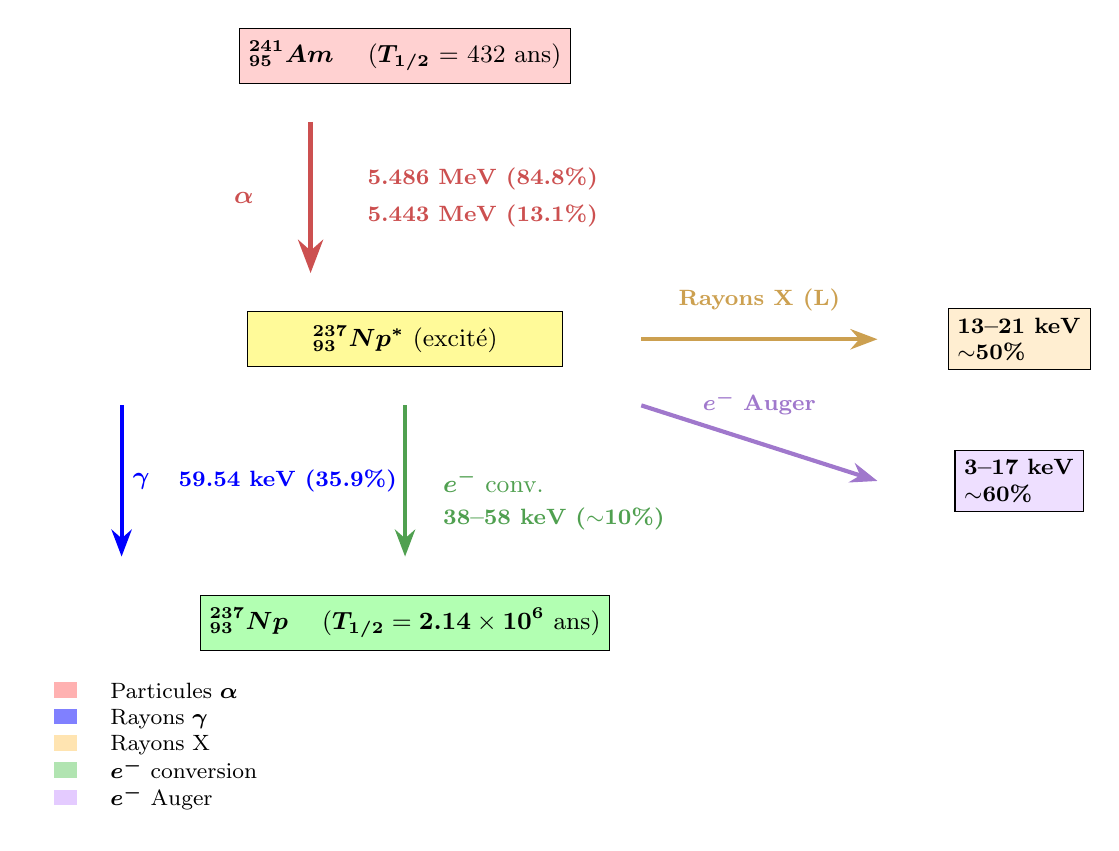
\begin{tikzpicture}[
    scale=1.2,
    every node/.style={font=\small},
    level/.style={draw, minimum width=4cm, minimum height=0.7cm},
    arrow/.style={->, thick, >=Stealth}
]

% Am-241
\node[level, fill=alphacolor!30] (Am) at (0, 8) {$\bm{^{241}_{95}Am}$ \quad ($\bm{T_{1/2}}$ = 432 ans)};

% Flèches alpha
\draw[arrow, alphacolor!80!black, line width=2pt] (-1, 7.3) -- (-1, 5.7);
\node[alphacolor!80!black, left] at (-1.5, 6.5) {$\bm{\alpha}$};
\node[alphacolor!80!black, right, font=\footnotesize] at (-0.5, 6.7) {\textbf{5.486 MeV (84.8\%)}};
\node[alphacolor!80!black, right, font=\footnotesize] at (-0.5, 6.3) {\textbf{5.443 MeV (13.1\%)}};

% Np-237 excité
\node[level, fill=yellow!40] (Np_ex) at (0, 5) {$\bm{^{237}_{93}}$$\bm{Np^*}$ (excité)};

% Branche gamma
\draw[arrow, blue, line width=1.5pt] (-3.0, 4.3) -- (-3.0, 2.7);
\node[blue, left] at (-2.6, 3.5) {$\bm{\gamma}$};
\node[blue, right, font=\footnotesize] at (-2.5, 3.5) {\textbf{59.54 keV (35.9\%)}};

% Branche conversion
\draw[arrow, electroncolor!80!black, line width=1.5pt] (0, 4.3) -- (0, 2.7);
\node[electroncolor!80!black, right] at (0.3, 3.5) {$\bm{e^-}$ conv.};
\node[electroncolor!80!black, right, font=\footnotesize] at (0.3, 3.1) {\textbf{38--58 keV ($\sim$10\%)}};

% Np-237 fondamental
\node[level, fill=green!30] (Np) at (0, 2) {$\bm{^{237}_{93}}\bm{Np}$ \quad ($\bm{T_{1/2}} = \bm{2.14}\times\bm{10^6}$ ans)};

% Rayons X (à droite)
\draw[arrow, xraycolor!80!black, line width=1.5pt] (2.5, 5) -- (5, 5);
\node[xraycolor!80!black, above, font=\footnotesize] at (3.75, 5.2) {\textbf{Rayons X (L)}};
\node[draw, fill=xraycolor!30, font=\footnotesize, align=left] at (6.5, 5) {\textbf{13--21 keV}\\$\sim$\textbf{50\%}};

% Électrons Auger (à droite, plus bas)
\draw[arrow, augercolor!80!black, line width=1.5pt] (2.5, 4.3) -- (5, 3.5);
\node[augercolor!80!black, above, font=\footnotesize] at (3.75, 4.1) {$\bm{e^-}$ \textbf{Auger}};
\node[draw, fill=augercolor!30, font=\footnotesize, align=left] at (6.5, 3.5) {\textbf{3--17 keV}\\$\sim$\textbf{60\%}};

% Légende
\node[anchor=north west, font=\footnotesize] at (-4, 1.5) {
\begin{tabular}{cl}
\tikz\fill[alphacolor!50] (0,0) rectangle (0.3,0.2); & Particules $\bm{\alpha}$ \\
\tikz\fill[blue!50] (0,0) rectangle (0.3,0.2); & Rayons $\bm{\gamma}$ \\
\tikz\fill[xraycolor!50] (0,0) rectangle (0.3,0.2); & Rayons X \\
\tikz\fill[electroncolor!50] (0,0) rectangle (0.3,0.2); & $\bm{e^-}$ conversion \\
\tikz\fill[augercolor!50] (0,0) rectangle (0.3,0.2); & $\bm{e^-}$ Auger \\
\end{tabular}
};

\end{tikzpicture}
\captionsetup{labelformat=empty}
\caption{\footnotesize Schéma de désintégration complet de l'Am-241}
 \end{figure}

\clearpage

\normalsize
\noindent \begin{mdframed}[backgroundcolor=orange!20]
\subsection{\color{blue}\textbf{Résumé des émissions}\color{black}}
\end{mdframed}
\footnotesize
\medskip

\begin{table}[H]
\centering
\caption{\footnotesize Types de particules émises par l'Am-241}
\renewcommand{\arraystretch}{1.4}
\begin{tabular}{l c c c c}
\toprule
\rowcolor{headercolor!30}
\footnotesize \textbf{Type de particule} &\footnotesize \textbf{Émis ?} &\footnotesize \textbf{Énergie typique} &\footnotesize \textbf{Intensité} & \textbf{Parcours (eau)} \\
\midrule
\rowcolor{alphacolor!30}
\footnotesize \textbf{Alpha ($\alpha$)} &\footnotesize \cmark \textbf{oui} &\footnotesize 5.49 MeV &\footnotesize $\sim$100\% &\footnotesize $\sim$40 µm \\
\rowcolor{gammacolor!30}
\footnotesize \textbf{Gamma ($\gamma$)} &\footnotesize \cmark oui &\footnotesize 59.5 keV &\footnotesize 35.9\% &\footnotesize $\sim$10 cm \\
\rowcolor{xraycolor!30}
\footnotesize \textbf{Rayons X} &\footnotesize \cmark oui &\footnotesize 13--21 keV &\footnotesize $\sim$50\% &\footnotesize $\sim$1 cm \\
\rowcolor{electroncolor!30}
\footnotesize \textbf{e$^-$ conversion} &\footnotesize \cmark oui &\footnotesize 38--58 keV &\footnotesize $\sim$10\% &\footnotesize $\sim$50 µm \\
\rowcolor{augercolor!30}
\footnotesize \textbf{e$^-$ Auger} &\footnotesize \cmark oui &\footnotesize 3--17 keV &\footnotesize $\sim$60\% &\footnotesize $\sim$10 µm \\
\midrule
\footnotesize Neutrons (n) &\footnotesize \xmark non &\footnotesize -- &\footnotesize -- &\footnotesize -- \\
\footnotesize Beta ($\beta^-$) &\footnotesize \xmark non &\footnotesize -- &\footnotesize -- &\footnotesize -- \\
\footnotesize Positrons ($\beta^+$) &\footnotesize \xmark non &\footnotesize -- &\footnotesize -- &\footnotesize -- \\
\bottomrule
\end{tabular}
\end{table}

\normalsize
\noindent \begin{mdframed}[backgroundcolor=orange!20]
\subsection{\color{blue}\textbf{Particules alpha ($\alpha$)}\color{black}}
\end{mdframed}
\footnotesize
\medskip

\begin{tcolorbox}[colback=blue!10,colframe=blue!70!black,title=\textbf{Émission alpha -- Mode de désintégration principal}]
L'Am-241 est un \color{blue}\textbf{émetteur alpha pur}\color{black}. Chaque désintégration produit une particule $\alpha$ (noyau d'hélium $^4_2$He$^{2+}$).
\end{tcolorbox}

\begin{table}[H]
\centering
\caption{\footnotesize Raies alpha de l'Am-241}
\renewcommand{\arraystretch}{1.3}
\begin{tabular}{c c c c}
\toprule
\rowcolor{alphacolor!30}
\footnotesize \textbf{Index} &\footnotesize \textbf{Énergie (MeV)} &\footnotesize \textbf{Intensité (\%)} &\footnotesize \textbf{Niveau Np excité} \\
\midrule
\rowcolor{alphacolor!20}
\footnotesize $\alpha_0$ &\footnotesize \textbf{5.486} &\footnotesize \textbf{84.8} &\footnotesize 59.54 keV \\
\rowcolor{alphacolor!15}
\footnotesize $\alpha_1$ &\footnotesize 5.443 &\footnotesize 13.1 &\footnotesize 103.0 keV \\
\footnotesize $\alpha_2$ &\footnotesize 5.388 &\footnotesize 1.6 &\footnotesize 158.5 keV \\
\footnotesize $\alpha_3$ &\footnotesize 5.545 &\footnotesize 0.34 &\footnotesize 0 keV (fondamental) \\
\footnotesize $\alpha_4$ &\footnotesize 5.512 &\footnotesize 0.20 &\footnotesize 33.2 keV \\
\midrule
\multicolumn{2}{c}{\footnotesize \textbf{TOTAL}} &\footnotesize \textbf{100.0} & \\
\bottomrule
\end{tabular}
\end{table}

\begin{tcolorbox}[colback=blue!10,colframe=blue,title=\textbf{Important pour la dosimétrie}]
\noindent Les particules $\alpha$ sont généralement \color{blue}\textbf{arrêtées par l'encapsulation}\color{black} de la source. Elles ne contribuent pas à la dose externe sauf en cas de contamination interne.
\end{tcolorbox}


\begin{mdframed}[backgroundcolor=orange!20]
\subsection{\color{blue}\textbf{Rayonnement gamma ($\gamma$)}\color{black}}
\end{mdframed}
\footnotesize
\medskip

\begin{tcolorbox}[colback=blue!10,colframe=blue!70!black,title=\textbf{Émission gamma -- Désexcitation du $^{237}$Np$^*$}]
Après émission $\alpha$, le noyau fils $^{237}$Np est dans un état excité. Il se désexcite par émission de rayons $\gamma$.
\end{tcolorbox}

\begin{table}[H]
\centering
\captionsetup{labelformat=empty}
\caption{\footnotesize Raies gamma de l'Am-241}
\renewcommand{\arraystretch}{1.3}
\begin{tabular}{c c c c}
\toprule
\rowcolor{gammacolor!30}
\footnotesize \textbf{Index} &\footnotesize \textbf{Énergie (keV)} &\footnotesize \textbf{Intensité (\%)} &\footnotesize \textbf{Commentaire} \\
\midrule
\rowcolor{gammacolor!25}
\footnotesize $\gamma_1$ &\footnotesize \textbf{59.54} &\footnotesize \textbf{35.90} &\footnotesize \textbf{Raie principale} \\
\rowcolor{gammacolor!15}
\footnotesize $\gamma_2$ &\footnotesize 26.34 &\footnotesize 2.40 &\footnotesize Secondaire \\
\footnotesize $\gamma_3$ &\footnotesize 33.20 &\footnotesize 0.126 &\footnotesize Faible \\
\footnotesize $\gamma_4$ &\footnotesize 43.42 &\footnotesize 0.073 &\footnotesize Faible \\
\footnotesize $\gamma_5$ &\footnotesize 55.56 &\footnotesize 0.018 &\footnotesize Très faible \\
\footnotesize $\gamma_6$ &\footnotesize 69.76 &\footnotesize 0.021 &\footnotesize Très faible \\
\footnotesize $\gamma_7$ &\footnotesize 98.97 &\footnotesize 0.0203 &\footnotesize Très faible \\
\footnotesize $\gamma_8$ &\footnotesize 102.98 &\footnotesize 0.0195 &\footnotesize Très faible \\
\footnotesize $\gamma_9$ &\footnotesize 125.30 &\footnotesize 0.0041 &\footnotesize Très faible \\
\midrule
\multicolumn{2}{c}{\footnotesize \textbf{TOTAL $\gamma$}} &\footnotesize \textbf{38.58} & \\
\bottomrule
\end{tabular}
\end{table}


\begin{mdframed}[backgroundcolor=orange!20]
\subsection{\color{blue}\textbf{Rayons X (fluorescence L du Neptunium)}\color{black}}
\end{mdframed}
\footnotesize
\medskip

\begin{tcolorbox}[colback=blue!20,colframe=blue!70!black,title=\textbf{Rayons X -- Réarrangement électronique}]
La conversion interne crée une lacune dans les couches électroniques du Np. Le réarrangement produit des rayons X caractéristiques (raies L).
\end{tcolorbox}

\begin{table}[H]
\centering
\captionsetup{labelformat=empty}
\caption{\footnotesize Raies X du Neptunium (couche L)}
\renewcommand{\arraystretch}{1.25}
\begin{tabular}{c c c c c}
\toprule
\rowcolor{xraycolor!40}
\footnotesize \textbf{Index} &\footnotesize \textbf{Raie} &\footnotesize \textbf{Énergie (keV)} &\footnotesize \textbf{Intensité (\%)} &\footnotesize \textbf{Transition} \\
\midrule
\rowcolor{xraycolor!20}
\footnotesize X1 &\footnotesize L$\ell$ &\footnotesize 11.89 &\footnotesize 0.84 &\footnotesize L$_3$--M$_1$ \\
\rowcolor{xraycolor!30}
\footnotesize X2 &\footnotesize L$\alpha_2$ &\footnotesize 13.93 &\footnotesize 13.0 &\footnotesize L$_3$--M$_4$ \\
\rowcolor{xraycolor!30}
\footnotesize X3 &\footnotesize L$\alpha_1$ &\footnotesize 13.95 &\footnotesize 13.0 &\footnotesize L$_3$--M$_5$ \\
\rowcolor{xraycolor!15}
\footnotesize X4 &\footnotesize L$\eta$ &\footnotesize 15.86 &\footnotesize 0.47 &\footnotesize L$_2$--M$_1$ \\
\rowcolor{xraycolor!25}
\footnotesize X5 &\footnotesize L$\beta_6$ &\footnotesize 16.84 &\footnotesize 3.4 &\footnotesize L$_3$--N$_1$ \\
\rowcolor{xraycolor!25}
\footnotesize X6 &\footnotesize L$\beta_1$ &\footnotesize 17.06 &\footnotesize 6.5 &\footnotesize L$_2$--M$_4$ \\
\rowcolor{xraycolor!25}
\footnotesize X7 &\footnotesize L$\beta_2$ &\footnotesize 17.75 &\footnotesize 5.2 &\footnotesize L$_3$--N$_4,5$ \\
\rowcolor{xraycolor!20}
\footnotesize X8 &\footnotesize L$\beta_3$ &\footnotesize 17.99 &\footnotesize 1.0 &\footnotesize L$_1$--M$_3$ \\
\rowcolor{xraycolor!25}
\footnotesize X9 &\footnotesize L$\gamma_1$ &\footnotesize 20.77 &\footnotesize 4.9 &\footnotesize L$_2$--N$_4$ \\
\rowcolor{xraycolor!20}
\footnotesize X10 &\footnotesize L$\gamma_2$ &\footnotesize 21.10 &\footnotesize 1.1 &\footnotesize L$_1$--N$_2$ \\
\rowcolor{xraycolor!15}
\footnotesize X11 &\footnotesize L$\gamma_3$ &\footnotesize 21.34 &\footnotesize 0.32 &\footnotesize L$_1$--N$_3$ \\
\midrule
\multicolumn{3}{c}{\footnotesize\textbf{TOTAL X (L)}} &\footnotesize \textbf{49.73} &\footnotesize \\
\bottomrule
\end{tabular}
\end{table}

\normalsize
\noindent \begin{mdframed}[backgroundcolor=orange!20]
\subsection{\color{blue}\textbf{Tableau du pourcentage d'absorption des raies Am-241 dans l'eau // Épaisseurs : 3 mm, 5 mm, 10 mm}\color{black}}
\end{mdframed}
\footnotesize
\medskip


\begin{table}[H]
\centering
\captionsetup{labelformat=empty}
\caption{\footnotesize Pourcentage d'absorption des raies X et $\gamma$ de l'Am-241 dans l'eau}
\begin{tabular}{@{}l c c c c c c@{}}
\toprule
\footnotesize\textbf{Raie} &\footnotesize \textbf{Énergie} &\footnotesize \textbf{Intensité} &\footnotesize $\bm{\mu/\rho}$ &\footnotesize \textbf{Abs. 3mm} &\footnotesize \textbf{Abs. 5mm} &\footnotesize \textbf{Abs. 10mm} \\
 &\footnotesize (keV) &\footnotesize (\%) &\footnotesize (cm$^2$/g) &\footnotesize (\%) &\footnotesize (\%) &\footnotesize (\%) \\
\midrule
\multicolumn{7}{c}{\footnotesize\textit{Rayons X du Neptunium (L X-rays)}} \\
\midrule
\footnotesize Np L$\ell$ X-ray &\footnotesize 11.89 &\footnotesize 0.84 &\footnotesize 3.250 &\footnotesize 62.28 &\footnotesize 80.30 & 96.12 \\
\rowcolor{yellow!20}
\footnotesize Np L$\alpha$ X-ray &\footnotesize 13.93 &\footnotesize 13.00 &\footnotesize 2.067 &\footnotesize 46.21 &\footnotesize 64.42 & 87.34 \\
\footnotesize Np L$\beta_1$ X-ray &\footnotesize 17.06 &\footnotesize 6.00 &\footnotesize 1.209 &\footnotesize 30.42 &\footnotesize 45.37 & 70.16 \\
\rowcolor{yellow!20}
\footnotesize Np L$\beta_2$ X-ray &\footnotesize 17.75 &\footnotesize 11.90 &\footnotesize 1.094 &\footnotesize 27.98 &\footnotesize 42.13 & 66.51 \\
\footnotesize Np L$\gamma$ X-ray &\footnotesize 20.78 &\footnotesize 4.90 &\footnotesize 0.753 &\footnotesize 20.22 &\footnotesize 31.37 &\footnotesize 52.91 \\
\midrule
\multicolumn{7}{c}{\footnotesize \textit{Rayons gamma}} \\
\midrule
\footnotesize $\gamma$ &\footnotesize 26.34 & \footnotesize2.40 &\footnotesize 0.481 &\footnotesize 13.43 &\footnotesize 21.36 &\footnotesize 38.16 \\
\footnotesize $\gamma$ &\footnotesize 33.20 &\footnotesize 0.12 &\footnotesize 0.334 &\footnotesize 9.52 &\footnotesize 15.36 &\footnotesize 28.37 \\
\footnotesize $\gamma$ &\footnotesize 43.42 &\footnotesize 0.07 &\footnotesize 0.252 &\footnotesize 7.29 &\footnotesize 11.85 &\footnotesize 22.30 \\
\rowcolor{yellow!20}
\footnotesize $\gamma$ \textbf{(principale)} &\footnotesize 59.54 &\footnotesize \textbf{35.90} &\footnotesize 0.207 &\footnotesize 6.01 &\footnotesize 9.82 &\footnotesize 18.68 \\
\midrule
\footnotesize \textbf{Moyenne pond.} & -- & -- & -- &\footnotesize \textbf{20.2} &\footnotesize \textbf{29.8} &\footnotesize \textbf{46.0} \\
\bottomrule
\end{tabular}
\end{table}
\footnotesize
\noindent \textbf{Source :} Am-241 $\rightarrow$ Np-237 + $\bm{\alpha}$ + $\bm{\gamma} + \bm{X}$ \quad ($\bm{T_{1/2}}$ = 432.6 ans) \\
\noindent \textbf{Formule :} Absorption (\%) $= [\bm{1} - \exp(-\bm{\mu} \times \bm{x})] \times 100$ \\
\noindent \textbf{Données :} Coefficients $\bm{\mu}/\bm{\rho}$ interpolés des données NIST XCOM \\
\noindent \textbf{Note :} Lignes surlignées = raies principales

\normalsize
\noindent \begin{mdframed}[backgroundcolor=orange!20]
\subsection{\color{blue}\textbf{Comparaison Am-241 vs Eu-152}\color{black}}
\end{mdframed}
\footnotesize
\medskip

\begin{table}[H]
\centering
\captionsetup{labelformat=empty}
\caption{\footnotesize Comparaison de l'absorption Am-241 vs Eu-152 dans l'eau}
\begin{tabular}{@{}l c c c c@{}}
\toprule
\footnotesize \textbf{Source} &\footnotesize \textbf{Gamme d'énergie} &\footnotesize \textbf{Abs. 3mm} &\footnotesize \textbf{Abs. 5mm} &\footnotesize \textbf{Abs. 10mm} \\
 &\footnotesize (keV) & (\%) & (\%) & (\%) \\
\midrule
\footnotesize \textbf{Am-241} &\footnotesize 12 -- 60 &\footnotesize \textbf{20.2} &\footnotesize \textbf{29.8} &\footnotesize \textbf{46.0} \\
\footnotesize \textbf{Eu-152} &\footnotesize 40 -- 1408 &\footnotesize 4.3 &\footnotesize 7.1 &\footnotesize 13.5 \\
\midrule
\footnotesize \textbf{Ratio Am/Eu} &\footnotesize -- &\footnotesize 4.7× &\footnotesize 4.2× &\footnotesize 3.4× \\
\bottomrule
\end{tabular}
\end{table}

\normalsize
\noindent \begin{mdframed}[backgroundcolor=orange!20]
\subsection{\color{blue}\textbf{Électrons de conversion interne}\color{black}}
\end{mdframed}
\footnotesize
\medskip

\begin{tcolorbox}[colback=blue!15,colframe=blue!70!black,title=\textbf{Conversion interne -- Alternative à l'émission gamma}]
Au lieu d'émettre un photon $\bm{\gamma}$, l'énergie de désexcitation peut être transférée directement à un électron des couches internes, qui est alors éjecté.

\vspace{0.1cm}
\noindent \color{blue}\textbf{Énergie de l'électron :}\color{black} $\bm{E_{e^-}} = \bm{E_\gamma} - \bm{E_{\text{liaison}}}$
\end{tcolorbox}

\begin{table}[H]
\centering
\captionsetup{labelformat=empty}
\caption{\footnotesize Électrons de conversion interne de l'Am-241 (transition 59.54 keV)}
\renewcommand{\arraystretch}{1.3}
\begin{tabular}{c c c c c}
\toprule
\rowcolor{electroncolor!30}
\footnotesize \textbf{Couche} &\footnotesize  \textbf{E$_{\text{liaison}}$ (keV)} &\footnotesize \textbf{E$_{e^-}$ (keV)} &\footnotesize \textbf{Intensité (\%)} & \textbf{Coefficient $\alpha$} \\
\midrule
\rowcolor{electroncolor!20}
\footnotesize $L_1$ &\footnotesize 22.4 &\footnotesize 37.1 &\footnotesize 2.0 &\footnotesize 0.056 \\
\rowcolor{electroncolor!20}
\footnotesize $L_2$ &\footnotesize 21.6 &\footnotesize 37.9 &\footnotesize 1.5 &\footnotesize 0.042 \\
\rowcolor{electroncolor!20}
\footnotesize $L_3$ &\footnotesize 17.6 &\footnotesize 41.9 &\footnotesize 4.5 &\footnotesize 0.125 \\
\rowcolor{electroncolor!15}
\footnotesize M (total) &\footnotesize $\sim$5 &\footnotesize $\sim$54 &\footnotesize 1.5 &\footnotesize 0.042 \\
\rowcolor{electroncolor!10}
\footnotesize N (total) &\footnotesize $\sim$1 &\footnotesize $\sim$58 &\footnotesize 0.3 &\footnotesize 0.008 \\
\midrule
\multicolumn{3}{c}{\footnotesize \textbf{TOTAL e$^-$ conversion}} &\footnotesize \textbf{$\sim$10} &\footnotesize $\alpha_{\text{tot}} \approx 0.28$ \\
\bottomrule
\end{tabular}
\end{table}

\noindent Le \color{blue}\textbf{coefficient de conversion interne}\color{black} $\bm{\alpha}$ est défini par :

\begin{equation*}
\bm{\alpha} = \frac{\bm{N_{e^-}}}{\bm{N_\gamma}} \approx \bm{0.28} \quad \text{pour la transition 59.54 keV}
\end{equation*}

\noindent Cela signifie que pour 100 désexcitations, $\sim$78 produisent un $\bm{\gamma}$ et $\sim$22 produisent un électron de conversion.

\normalsize
\noindent \begin{mdframed}[backgroundcolor=orange!20]
\subsection{\color{blue}\textbf{Électrons Auger}\color{black}}
\end{mdframed}
\footnotesize
\medskip

\begin{tcolorbox}[colback=blue!15,colframe=blue!70!black,title=\textbf{Effet Auger -- Cascade électronique}]
Après conversion interne ou émission X, une lacune est créée dans les couches internes. Le réarrangement peut produire soit un rayon X, soit un électron Auger (processus non radiatif).
\end{tcolorbox}

\begin{table}[H]
\centering
\captionsetup{labelformat=empty}
\caption{\footnotesize Électrons Auger de l'Am-241}
\renewcommand{\arraystretch}{1.3}
\begin{tabular}{c c c c}
\toprule
\rowcolor{augercolor!30}
\footnotesize \textbf{Type} &\footnotesize \textbf{Énergie (keV)} &\footnotesize \textbf{Intensité (\%)} &\footnotesize \textbf{Origine} \\
\midrule
\rowcolor{augercolor!20}
\footnotesize Auger L (LMM) &\footnotesize 11--17 &\footnotesize $\sim$12 &\footnotesize Lacune couche L \\
\rowcolor{augercolor!15}
\footnotesize Auger M (MNN) &\footnotesize 3--4 &\footnotesize $\sim$40 &\footnotesize Lacune couche M \\
\rowcolor{augercolor!10}
\footnotesize Auger N & $<$1 &\footnotesize $\sim$10 &\footnotesize Lacune couche N \\
\rowcolor{augercolor!10}
\footnotesize Coster-Kronig &\footnotesize 1--5 &\footnotesize $\sim$5 &\footnotesize Transitions intra-couche \\
\midrule
\multicolumn{2}{c}{\footnotesize \textbf{TOTAL Auger}} &\footnotesize \textbf{$\sim$60--70} &\footnotesize \\
\bottomrule
\end{tabular}
\end{table}

\normalsize
\noindent \color{blue}\textbf{Importance des électrons Auger}\color{black}
\footnotesize

\begin{itemize}
\item \textbf{Très nombreux :} $>$60 électrons Auger pour 100 désintégrations
\item \textbf{Basse énergie :} Majoritairement $<$20 keV
\item \textbf{Parcours court :} $<$10 µm dans les tissus
\item \textbf{Fort TEL :} Haute densité d'ionisation locale
\item \textbf{Radiotoxicité :} Très dangereux en contamination interne (dommages ADN locaux)
\end{itemize}

\normalsize
\noindent \begin{mdframed}[backgroundcolor=orange!20]
\subsection{\color{blue}\textbf{Bilan par désintégration}\color{black}}
\end{mdframed}
\footnotesize
\medskip


\begin{table}[H]
\centering
\captionsetup{labelformat=empty}
\caption{\footnotesize Bilan des émissions pour 100 désintégrations d'Am-241}
\renewcommand{\arraystretch}{1.4}
\begin{tabular}{l c c c}
\toprule
\rowcolor{headercolor!30}
\footnotesize \textbf{Type de particule} &\footnotesize \textbf{Nombre / 100 désint.} &\footnotesize \textbf{Énergie moyenne} &\footnotesize \textbf{Énergie totale} \\
\midrule
\rowcolor{alphacolor!20}
\footnotesize Particules $\alpha$ &\footnotesize 100 &\footnotesize 5.48 MeV &\footnotesize 548 MeV \\
\rowcolor{gammacolor!20}
\footnotesize Photons $\gamma$ &\footnotesize 39 &\footnotesize 57 keV &\footnotesize 2.2 MeV \\
\rowcolor{xraycolor!20}
\footnotesize Rayons X &\footnotesize 50 &\footnotesize 16 keV & \footnotesize0.8 MeV \\
\rowcolor{electroncolor!20}
\footnotesize $e^-$ conversion &\footnotesize 10 &\footnotesize 45 keV &\footnotesize 0.45 MeV \\
\rowcolor{augercolor!20}
\footnotesize $e^-$ Auger &\footnotesize 65 &\footnotesize 8 keV &\footnotesize 0.5 MeV \\
\midrule
\footnotesize \textbf{TOTAL} &\footnotesize \textbf{264 particules} & \footnotesize-- & \footnotesize\textbf{$\sim$552 MeV} \\
\bottomrule
\end{tabular}
\end{table}

\begin{tcolorbox}[colback=blue!10,colframe=blue,title=\textbf{Points clés}]
\begin{itemize}
\item L'énergie est dominée par les \color{blue}\textbf{particules $\bm{}\alpha$}\color{black} (99.3\% de l'énergie totale)
\item Les $\alpha$ sont \color{blue}\textbf{arrêtées localement}\color{black} (parcours $\sim$40 µm)
\item La \color{blue}\textbf{dose externe}\color{blue} est due principalement au $\bm{\gamma}$ 59.54 keV
\item En \color{blue}\textbf{contamination interne}\color{black}, les $\bm{\alpha}$ et électrons Auger sont très radiotoxiques
\end{itemize}
\end{tcolorbox}

\normalsize
\noindent \begin{mdframed}[backgroundcolor=orange!20]
\subsection{\color{blue}\textbf{Implications pour la simulation et la dosimétrie}\color{black}}
\end{mdframed}
\footnotesize
\medskip

\normalsize
\noindent \color{blue}\textbf{Simulation Monte Carlo}\color{black}
\footnotesize

\noindent Pour une simulation Geant4 de l'Am-241, il faut considérer :

\begin{table}[H]
\centering
\captionsetup{labelformat=empty}
\caption{\footnotesize Recommandations pour simulation Geant4}
\renewcommand{\arraystretch}{1.3}
\begin{tabular}{l l l}
\toprule
\rowcolor{headercolor!30}
\footnotesize \textbf{Application} &\footnotesize \textbf{Particules à simuler} &\footnotesize \textbf{Commentaire} \\
\midrule
\footnotesize Dose externe (source encapsulée) &\footnotesize $\gamma$ + X &\footnotesize $\alpha$ arrêtées par encapsulation \\
\footnotesize Calibration détecteur &\footnotesize $\gamma$ 59.54 keV &\footnotesize Raie principale uniquement \\
\footnotesize Spectrométrie complète &\footnotesize $\gamma$ + X &\footnotesize Spectre complet \\
\bottomrule
\end{tabular}
\end{table}

\normalsize
\noindent \color{blue}\textbf{Comparaison dosimétrique Am-241 vs Eu-152}\color{black}
\footnotesize

\begin{table}[H]
\centering
\captionsetup{labelformat=empty}
\caption{\footnotesize Comparaison des sources pour irradiation externe}
\renewcommand{\arraystretch}{1.3}
\begin{tabular}{l c c}
\toprule
\rowcolor{headercolor!30}
\footnotesize \textbf{Paramètre} &\footnotesize \textbf{Am-241} &\footnotesize \textbf{Eu-152} \\
\midrule
\footnotesize Énergie $\gamma$ principale &\footnotesize 59.54 keV &\footnotesize 344 keV \\
\footnotesize Intensité $\gamma$ &\footnotesize  35.9\% &\footnotesize 26.6\% \\
\footnotesize Pénétration dans l'eau &\footnotesize $\sim$10 cm &\footnotesize $\sim$50 cm \\
\footnotesize Dose en profondeur &\footnotesize Faible (basse énergie) &\footnotesize Élevée (haute énergie) \\
\footnotesize Blindage nécessaire &\footnotesize Léger (quelques mm Pb) &\footnotesize Important (plusieurs cm Pb) \\
\footnotesize \textbf{Application typique} &\footnotesize \textbf{Dose superficielle} &\footnotesize \textbf{Dose en profondeur} \\
\bottomrule
\end{tabular}
\end{table}


\end{document}
